\documentclass[12pt]{article}
\usepackage{url}
\usepackage{graphicx}
\usepackage{float}
\usepackage{amsmath}
\usepackage{amssymb}
\usepackage{pdfpages}
\usepackage{subcaption}
\usepackage{hyperref}
\begin{document}

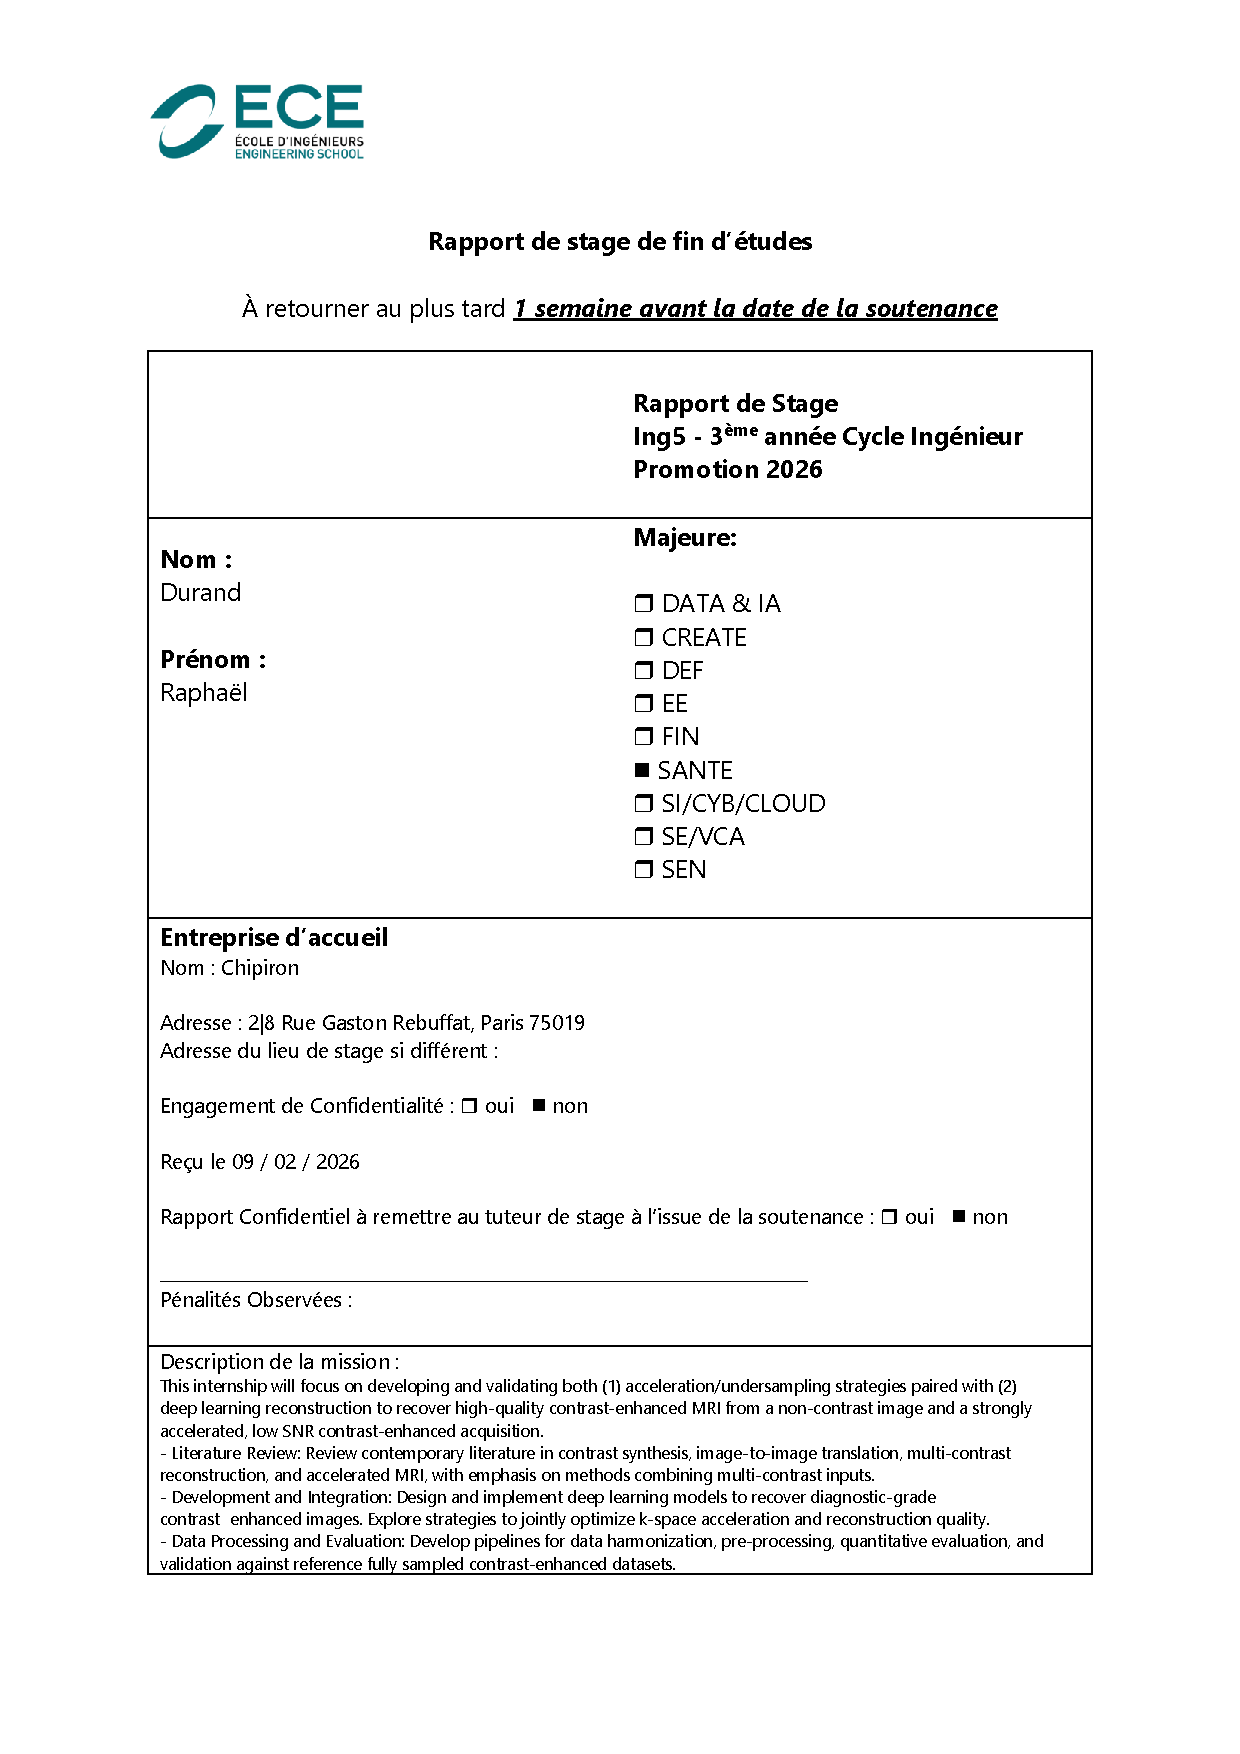
\includepdf[pages=1]{image/Page de garde Promo 2026.pdf}

\tableofcontents
\newpage

\section{Project Presentation}
\subsection{Company Context}

\subsubsection{Chipiron global context}
Chipiron is a French deeptech company founded in 2020 by Dimitri Labat and Evan Kervella. 
Based in the 19th arrondissement of Paris, the company brings together around 30 employees from multidisciplinary backgrounds, including MRI physics, hardware engineering, software development, and artificial intelligence.

Chipiron operates in the healthcare sector, more specifically in the field of medical imaging. 
The company is developing a new generation of ultra-low-field MRI systems designed to be lighter, more affordable, and easier to deploy than conventional MRI scanners.
Its initial clinical focus is breast imaging, with the aim of improving access to early cancer detection and screening.

Through its innovative approach combining advanced hardware and AI-driven image reconstruction techniques, Chipiron aims to make MRI examinations more accessible and ultimately transform the way medical imaging is delivered worldwide.
At Chipiron, it is believed that within the next decade, low-field MRI could become as routine as standard blood tests, enabling new opportunities in health monitoring and personalized medicine. 
Since its creation in 2020, the start-up has been working to overcome current limitations and position itself among the first companies to develop and manufacture low-field MRI systems (around 10~mT) dedicated to breast imaging.

\subsubsection{Epidemiology and Clinical Context}
Breast cancer is the most commonly diagnosed cancer among women worldwide \cite{iarc2025}. 
Based on current trends, 1 in 20 women will develop breast cancer in their lifetime, and among them, 30\% will die from the disease.
These numbers vary significantly between regions: in the United States, the incidence is higher, with 1 in 10 women developing breast cancer, but the mortality rate is approximately 16\%.
More concerning is the rapid increase in incidence among young women, with an annual growth of 2.1\% from 1990 to 2018 in Europe, for reasons that remain unclear to this day.
The good news is that early detection makes a major difference. 
Stage I breast cancer has a 5-year survival rate above 98\% \cite{nbc_mammo}, whereas this rate drops below 70\% for stage III disease.
Tumor progression is highly heterogeneous, but the most aggressive forms can reach stage III in less than one year.

The American College of Radiology (ACR) recommends annual breast cancer screening for all women over the age of 40. 
Depending on individual risk factors, high-risk patients may be advised to undergo more frequent imaging even before this age.

\subsubsection{Breast Cancer Screening Pipeline with its Limitations}

The standard technique used for breast cancer screening is mammography. 
It is an established imaging modality that entered widespread clinical use in the 1960s \cite{komen_stats}. 
Since then, it has evolved considerably, from a basic 2D X-ray technique to digital breast tomosynthesis, which enables high-resolution 3D imaging of the breast.

Despite being relatively inexpensive, high-throughput, and highly sensitive in non-dense breast tissue, modern mammography has important limitations:

\begin{itemize}
    \item It is uncomfortable for patients, as it requires breast compression to obtain standardized image quality.
    \item It involves ionizing radiation, and cumulative exposure can be harmful.
    \item Most importantly, it is not sufficiently reliable. Sensitivity varies significantly depending on the technique, ranging from as low as 55\% to up to 90\% for more advanced methods.
    This can lead to a non-negligible number of false negatives.
    Specificity is generally higher, around 85\% to 95\%, which is less problematic in a screening context where minimizing false negatives is the priority.
\end{itemize}

The main reason behind the lack of sensitivity of mammography is the variability of breast anatomy between patients. 
In the United States, it is estimated \cite{org_breast} that more than 40\% of women over 40 years old have heterogeneous or extremely dense breast tissue. 
These patients are at higher risk of developing breast cancer, and mammography becomes more difficult to interpret because dense tissue can mask tumors, leading to an increased rate of false negatives, with approximately 1 in 8 breast cancers being missed \cite{pu2026}.
Despite its reduced performance in dense breast populations, mammography remains the standard method for population-wide breast cancer screening.

After a mammography examination, if a suspicious finding is detected or if breast density makes the exam inconclusive, the patient is typically referred to a second-line imaging modality. 
Depending on the clinical context, this may involve direct biopsy or additional imaging. 
Ultrasound is the most commonly used second-line technique due to its low cost and accessibility. 
When performed correctly, it can be highly effective. 
However, its performance remains strongly operator-dependent, resulting in variable sensitivity and specificity.

The last option in the diagnostic pathway is breast MRI, which is considered the most sensitive imaging modality. 
However, due to its high cost and operational constraints, it is still not widely accessible. 
The ACR recommends MRI primarily for high-risk patients, representing approximately 10 to 15\% of the population.
Factors contributing to this elevated risk include pathogenic genetic mutations, a strong family history of breast cancer, prior chest irradiation at a young age, and certain hereditary cancer syndromes such as Li-Fraumeni or Cowden syndrome \cite{syndrom2026}.
These women are usually advised to initiate MRI screening before the age of 30, in addition to conventional mammographic surveillance.

\subsubsection{Low-Field MRI Solution}
Chipiron chose to focus on magnetic resonance imaging (MRI) for breast imaging applications because, as discussed in the previous section, it represents the most advanced medical imaging modality.
High-field MRI provides a wide variety of soft tissue contrasts at millimetric resolution within a few minutes of acquisition.
Depending on the sequence used, MRI enables visualization of anatomical structures, vessels, tumors, lesions, and even subtle differences in temperature or chemical composition within muscles and internal organs. 
Some MRI sequences also allow monitoring of metabolic or functional activity. 
For these reasons, MRI is an essential tool for diagnosing many life-threatening diseases, monitoring treatment effectiveness, and enabling image-guided therapy and surgery.

In the context of breast cancer imaging, MRI can accurately detect tumors of only a few millimeters in size, with a sensitivity higher than mammography, which remains the current gold standard for screening. 
Using contrast agent injection, MRI can also discriminate between benign and malignant lesions, reducing the number of false positives by approximately 77\% \cite{diag2026}.

Despite these advantages, MRI remains largely inaccessible worldwide. 
MRI systems typically weigh around five tons and require a magnetically shielded room, costly maintenance, and highly trained staff. 
They operate using strong magnetic fields generated by large superconducting electromagnets. 
Higher magnetic field strength generally leads to higher image quality for a given scan time.

For decades, MRI manufacturers have focused on increasing magnetic field strength as the main driver of image quality. 
Most clinical MRI systems operate at 1.5~T or 3~T, while research systems can reach up to 7~T, with fewer than 150 units deployed worldwide.

However, increasing field strength directly leads to larger, more expensive, and less accessible systems. 
Therefore, democratizing MRI requires achieving clinically relevant image quality at lower magnetic fields. 
This idea is not new: since the early days of MRI, engineers have attempted to build low-field clinical systems. 
However, none of these efforts have yet achieved large-scale clinical adoption due to multiple technical and physical constraints.

In fact, MRI at low magnetic field strengths remains challenging. 
The lower field strength alone reduces the signal levels, leading to a lower signal-to-noise ratio (SNR).
The hardware is also less mature and optimized than that of conventional high-field scanners, leading to increased noise and artifacts but also affecting robustness.
Since SNR is a major determinant of image quality, it needs to be improved by repeating acquisitions, leading to longer exams or alternatively to reduced image resolution as a trade-off to save time.

Moreover, magnetic field strength is by no means the only driver of image quality. 
Images produced on 1.5~T scanners have improved tremendously since the 1990s, largely thanks to major advances in hardware such as stronger and more sensitive receiver coils, improved gradient systems, and the advent of parallel imaging alongside software improvements, which are no less vital than hardware.
Finally, the use of AI in commercial MRI systems is very recent, even though it has been explored in academic research since the early days of deep learning.
The limited use of AI mainly comes from the difficulty of ensuring that it does not remove or invent structures in the images.
It is not easy to guarantee that the output is reliable and faithful to the original data. 
While AI brings flexibility, this also increases the need for additional controls to ensure robustness and consistency.
\subsubsection{Chipiron Current Position in Low-Field MRI Development}
% Chipiron position

\subsubsection{Industry Sector}
% Over companies working on MRI (hyperfine)
% Type of technologies
There are several major companies in the MRI market, such as Siemens Healthineers, GE HealthCare, Philips Healthcare, and Canon Medical Systems.
However, these companies mainly focus on high-field MRI systems, typically operating at 1.5~T or 3~T.
In recent years, they have also started to explore low-field MRI around 0.5~T with promising results, but this remains far above the 10~mT targeted by Chipiron.
These high-field MRI manufacturers are therefore not considered direct competitors to Chipiron.

Indeed, a 10~mT MRI scanner will never replace a 3~T MRI scanner.
High-field MRI will still be necessary, especially for the most complex clinical cases and simply for establishing a diagnosis, as low-field MRI would be used for screening only.
Low-field MRI is instead aimed at increasing accessibility and providing sufficient information for fast clinical decision-making in more routine or resource-limited settings.

For this reason, it is more relevant to look at companies developing low-field MRI systems, although there are currently only a few of them on the market.
The main pioneer in this field is Hyperfine, an American company that received Food and Drug Administration (FDA) clearance in 2021 for its portable MRI device called \textit{Swoop}.
The system operates at 64~mT and was designed mainly for rapid brain imaging and stroke assessment.
Thanks to advanced AI-based reconstruction methods, the image quality has improved significantly compared to traditional low-field reconstruction approaches.

Despite these impressive improvements, Hyperfine is still searching for a strong product-market fit. 
One difficulty is that many patients scanned with their system are elderly or have limited mobility.
This makes positioning inside the scanner more complicated than in standard high-field MRI systems, where patient positioning is facilitated by dedicated tables and controlled scanning environments.

In any case, Hyperfine and Chipiron target very different applications. 
Hyperfine mainly focuses on brain imaging, while Chipiron is focused on breast imaging.
% Industrials actors
The goal of Chipiron is to establish a strong and clearly defined use case, supported by sufficiently reliable technology, in order to attract major industrial partners who could potentially acquire or collaborate with the company. 
Once Chipiron obtains FDA clearance, it will not have the manufacturing capacity or infrastructure to produce MRI systems at scale. 
As a result, it will need to partner with large established manufacturers such as Siemens or GE HealthCare to enable large-scale production and distribution.


\subsubsection{Markets and Clients}

The market targeted by Chipiron is currently the United States. 
Obtaining FDA clearance is generally considered more straightforward than achieving CE marking in Europe. 
Moreover, it is easier to deploy and to identify potential buyers for the system, as the U.S. hospital system is more privately driven, making adoption decisions more decentralized.
In addition, the prevalence of dense breast tissue is higher in the U.S. \cite{densebreast} population than in Europe, which increases the risk of undetected malignant cancers and therefore strengthens the clinical need for improved breast imaging solutions.

Initially, Chipiron's objective is to commercialize low-field MRI systems for research institutes and small clinical facilities. 
Once the technology has demonstrated its reliability and clinical value, the company aims to expand its deployment on a larger scale by targeting hospitals and larger healthcare institutions.

\subsubsection{Products and Services}

The company's objective is to commercialize low-field MRI systems. To achieve this goal, Chipiron will rely on partnerships with manufacturing companies for the industrial production of the devices. 
Therefore, the main value provided by the company will be its expertise in both hardware development and software solutions, which constitute the core of its technological advantage.

\subsubsection{Strategic Objectives}

To commercialize a medical device, regulatory approval from the FDA is required. 
Therefore, Chipiron must successfully validate its clinical trials to obtain FDA clearance.

The clinical validation process would be divided into two main phases:

\begin{itemize}
    \item The first clinical phase would focus on assessing the overall image quality after gadolinium injection. 
    The objective would be to verify whether the contrast enhancement is visually detectable and whether the reconstructed images provide sufficient quality.
    
    \item The second clinical phase would involve another group of patients and would focus more specifically on dynamic contrast-enhanced MRI analysis, particularly the evaluation of wash-in and wash-out useful for the diagnostic.
\end{itemize}

Once the clinical validation phase is successfully completed, the initial commercialization strategy would target research institutes and small clinical facilities. 
This approach would allow the technology to demonstrate its reliability and clinical value in real-world conditions.

After establishing the performance and credibility of the MRI system, the objective would be to expand its adoption across larger healthcare institutions, including hospitals. 

\subsection{Hosting Department or Service}
Chipiron is organized into several departments, the main ones being the hardware team and the software team.
Our hosting department was the software team, within which we were part of the AI team.
The software team is composed of four people: Nina Gidel-Dissier, who is the AI Engineering Manager, and Guillaume Daval-Frérot and Angelo Franciosini, who were both our supervisors.

\begin{figure}[H]
    \centering
    \vspace{0.5cm}
    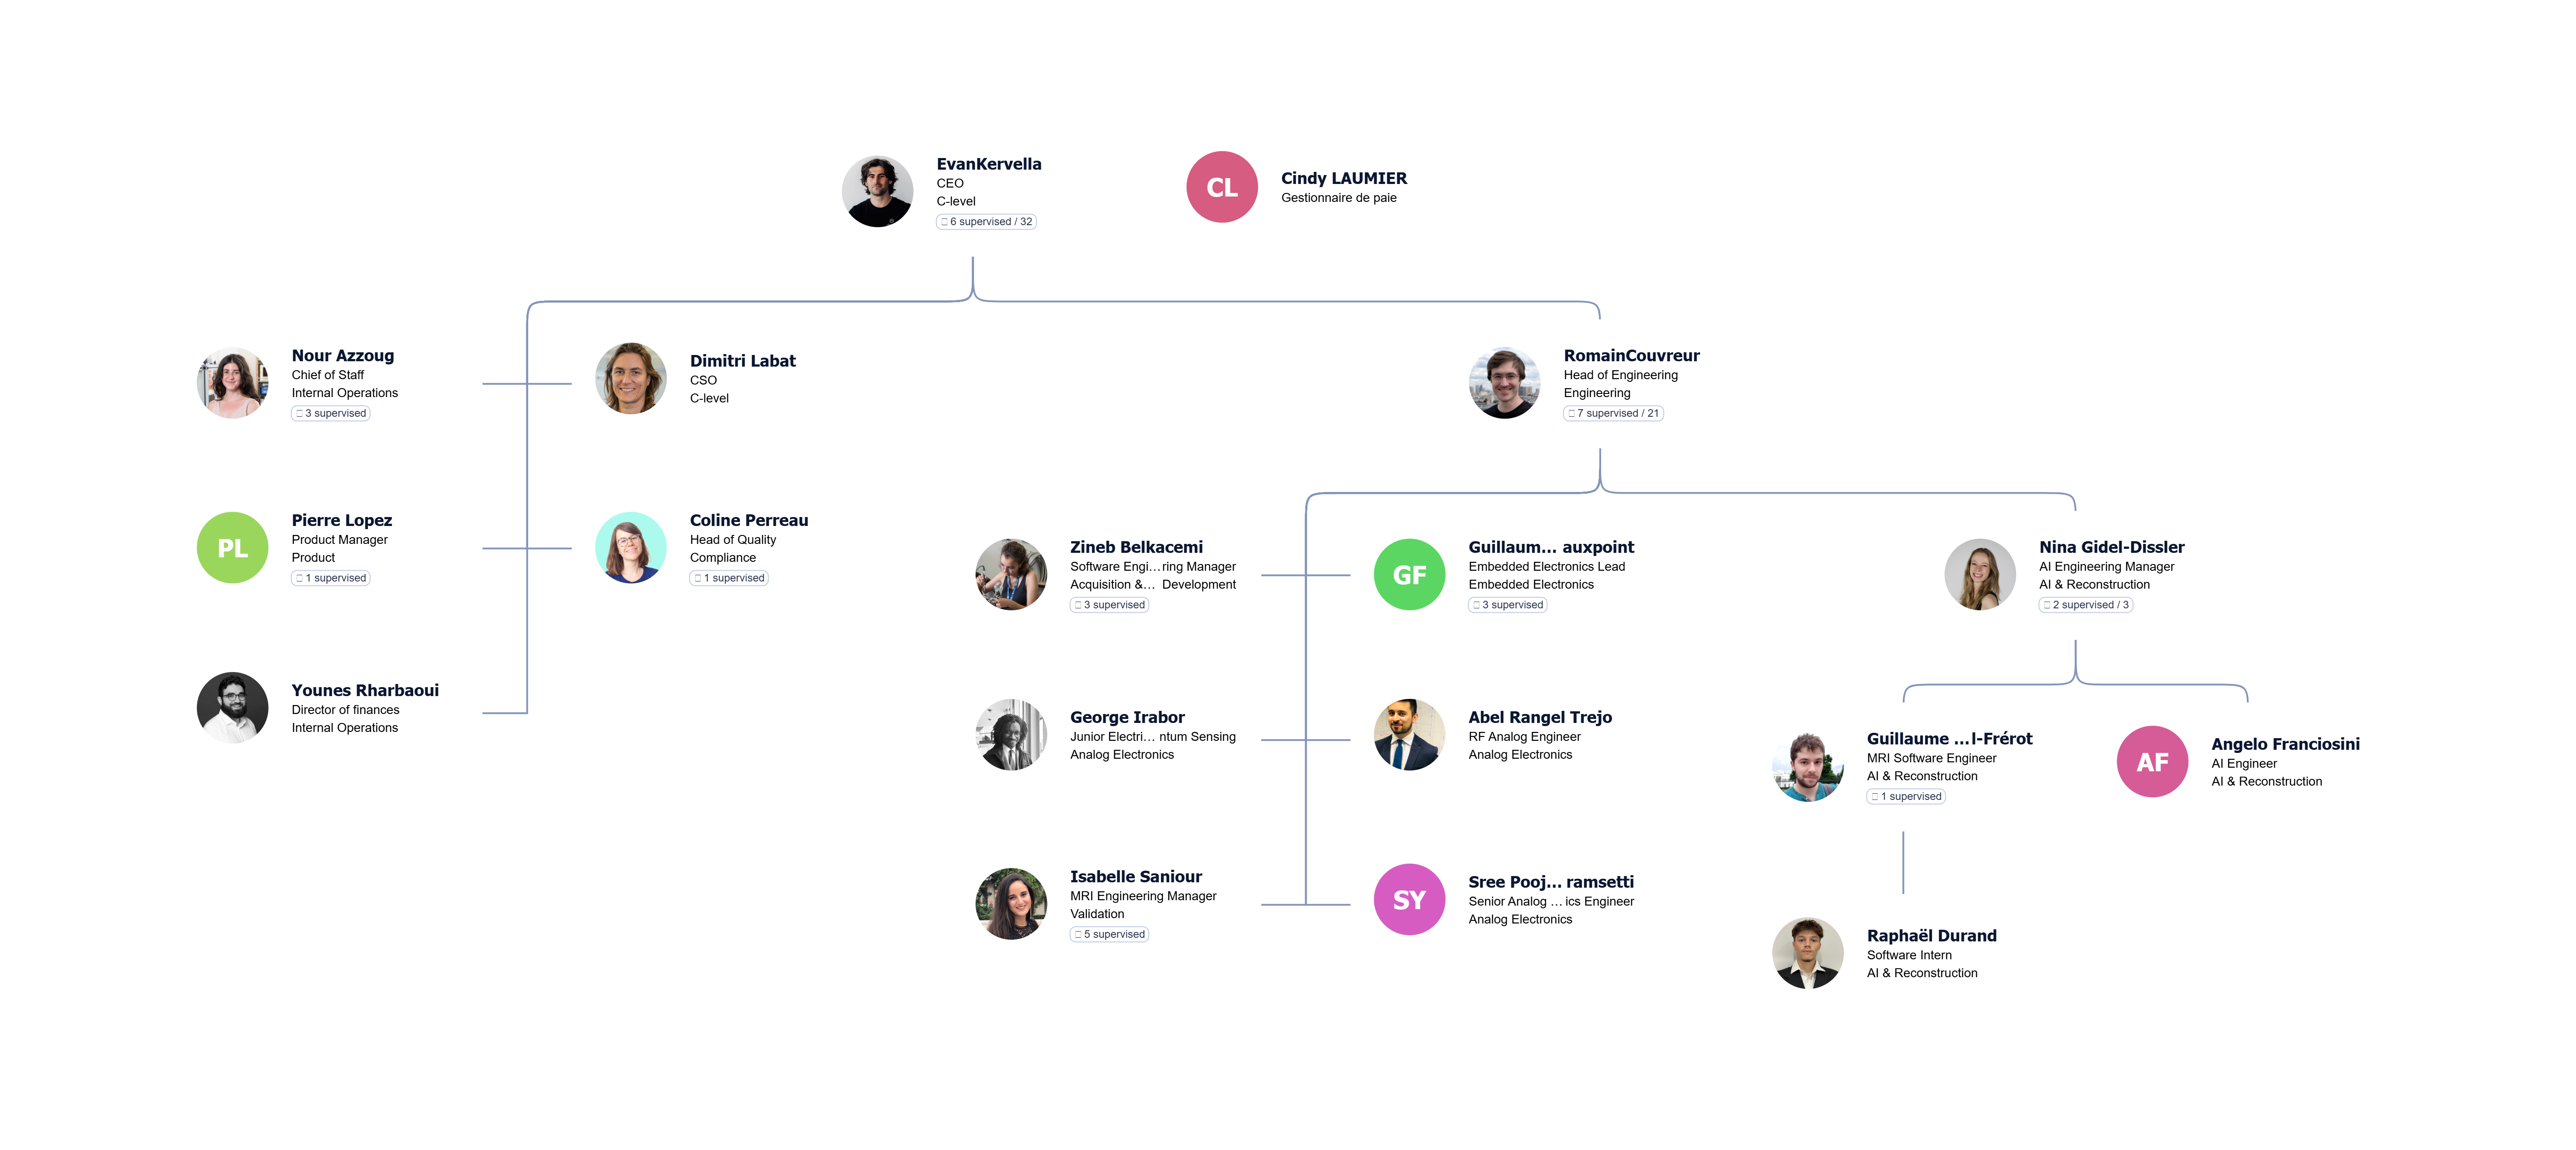
\includegraphics[width=0.75\textwidth]{image/Employees_Chart.png}
    \caption{Employees Chart}
    \label{fig:Employees Chart}
    \vspace{0.5cm}
\end{figure}

\subsection{Purpose of the Mission for the Company}

In MRI, contrast agents such as gadolinium are used to help determine whether a lesion is benign or malignant.
Gadolinium is injected into the bloodstream and circulates through the body.
It tends to accumulate in highly vascularized tissues, such as malignant lesions, making them appear brighter on MRI scans. 
Radiologists analyze the temporal evolution of the contrast enhancement, known as the dynamic contrast enhancement (DCE).
The objective is to observe how the signal intensity evolves over time after the injection of the contrast agent. 
A malignant lesion typically presents a rapid increase in signal intensity followed by a rapid decrease. 
This behavior is referred to as the \textit{wash-in/wash-out} phenomenon and is associated with a high probability of malignancy \cite{washinwashout}.
In contrast, a benign lesion generally shows a slower enhancement and tends to maintain a high signal intensity over a longer period of time, indicating a lower risk of malignancy.
For example, in Figure~\ref{fig:dynamic_curve}, the lesion is likely benign because the signal intensity decreases slowly over time after the initial contrast enhancement.
% Show an example of benign lesion and malign lesion

\begin{figure}[H]
    \centering
    \vspace{0.5cm}
    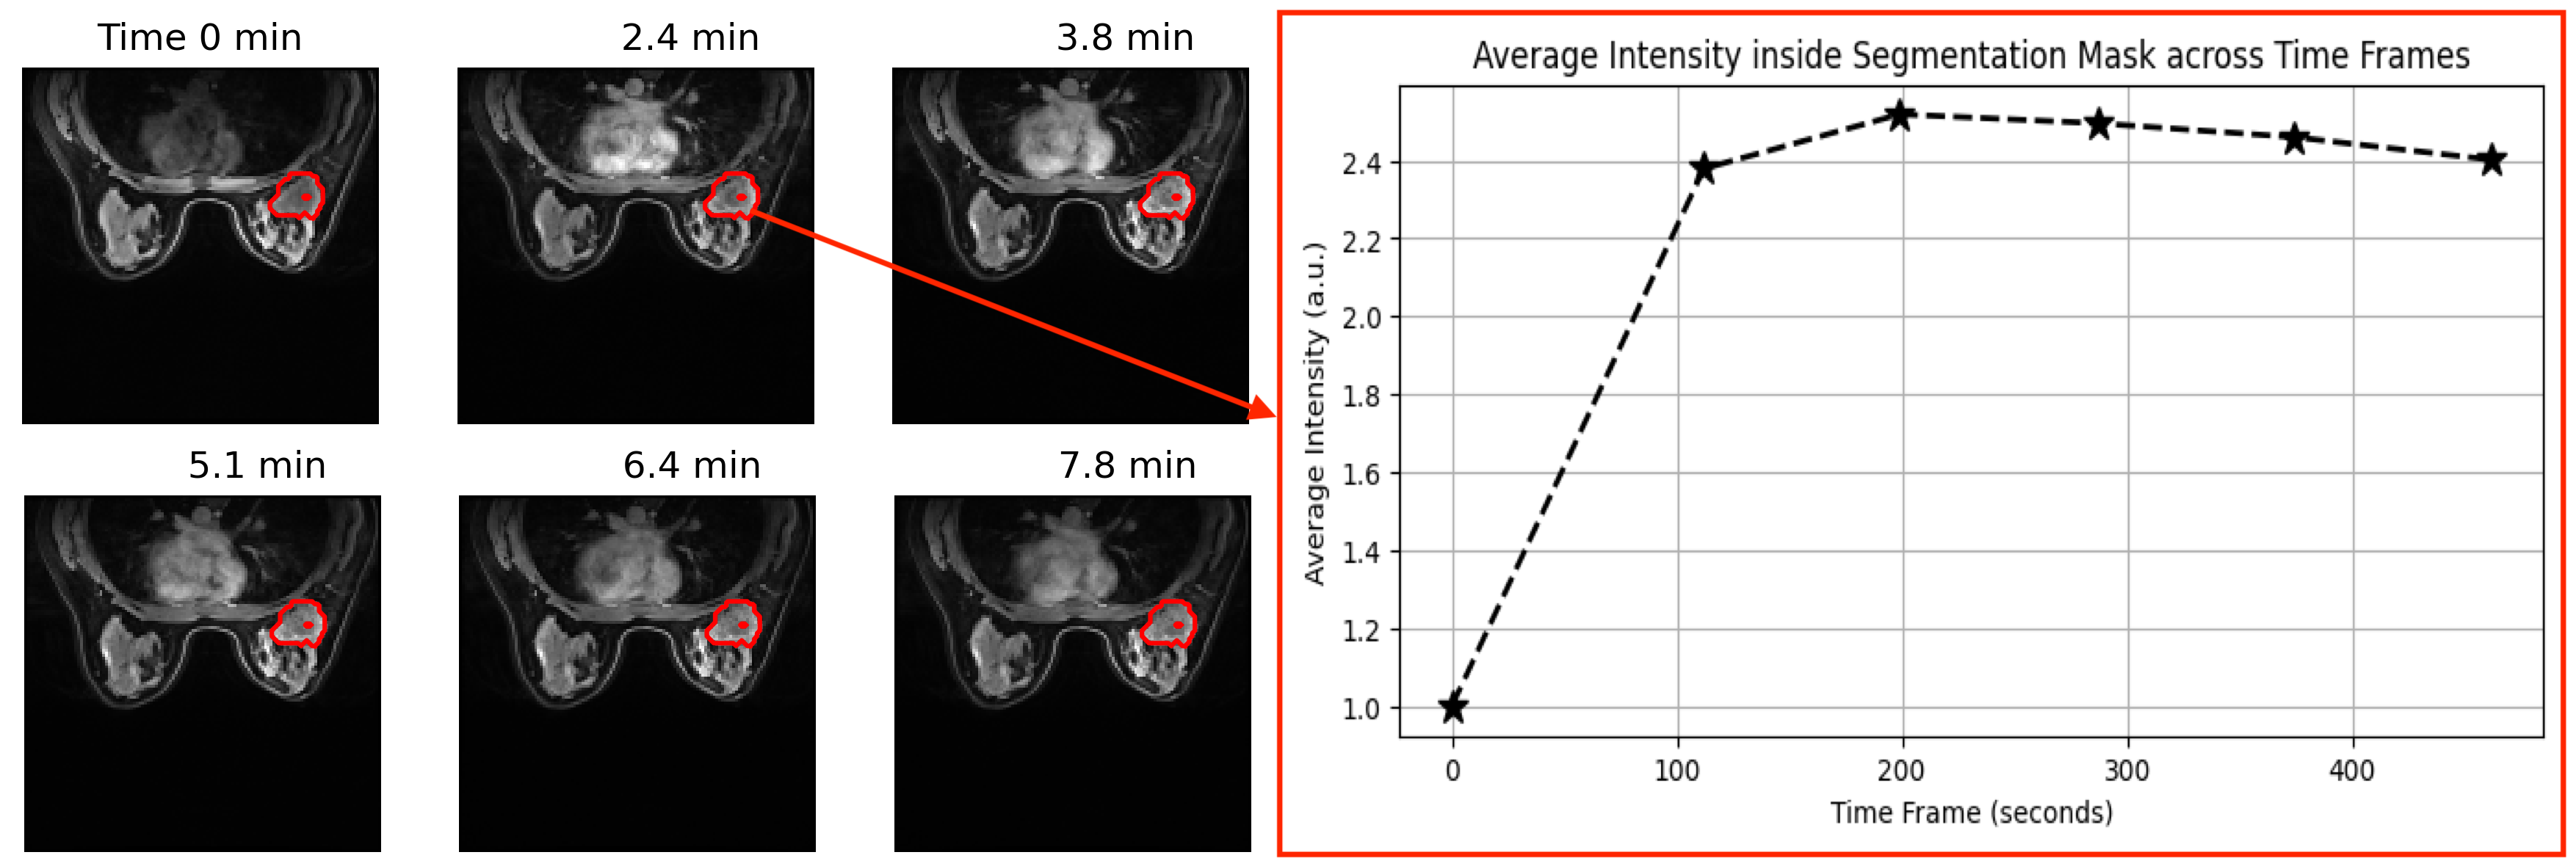
\includegraphics[width=0.75\textwidth]{image/example_curve.png}
    \caption{Dynamic contrast enhancement curves illustrating benign and malignant lesion behaviors}
    \label{fig:dynamic_curve}
    \vspace{0.5cm}
\end{figure}

The more aggressive the lesion is, the faster the acquisition must be in order to correctly capture the wash-in and wash-out dynamics.
Consequently, MRI acquisitions need to be accelerated. 
However, accelerating the acquisition process generally leads to a degradation in image quality.
More precisely, accelerating the acquisition means acquiring fewer samples in k-space, which is the frequency domain where the MRI signal is encoded.
By accelerating the acquisition, as explained earlier, the SNR decreases.
Therefore, the objective of this internship is to perform a feasibility study to evaluate different deep learning models capable of enhancing image quality after accelerated MRI acquisition, while preserving sufficient temporal and spatial information to accurately analyze the contrast enhancement dynamics over time.

\begin{figure}[H]
    \centering
    \vspace{0.5cm}
    
\includegraphics[width=0.75\textwidth]{\detokenize{image/Project summary.png}}
    \caption{Neural network helping on gaining acquisition time}
    \label{fig:Neural network helping on gaining acquisition time}
    \vspace{0.5cm}
\end{figure}

As illustrated in Figure~\ref{fig:Neural network helping on gaining acquisition time}, the goal of the neural network is to achieve the best possible trade-off between acquisition time and image quality, reducing scan time while preserving sufficient image quality.

Apart from working on deep learning models, it is also important to evaluate which trajectory configurations are optimal to achieve the fastest possible acquisition while preserving the best image quality and contrast enhancement.

\section{Corporate Social Responsibility (CSR) Policy}
Corporate Social Responsibility (CSR) refers to the responsibility of organizations for their impacts on society and the environment. 
According to ISO 26000, CSR is based on seven key principles:
accountability, transparency, ethical behavior, respect for stakeholder interests, respect for the rule of law, respect for international norms of behavior, and respect for human rights.

Chipiron integrates CSR into its development strategy.
As the company grows, it aims to make decisions that are responsible, transparent, and respectful of the people it works with.
The following principles guide the way we work.

\paragraph{Accountability}
\mbox{}\\

Chipiron takes responsibility for its decisions, its actions, and their impact on colleagues, partners, customers, and society.
It encourages ownership, continuous learning, and open discussions when mistakes happen, so that everyone can improve together.

\paragraph{Transparency}
\mbox{}\\

Chipiron strives to communicate openly and honestly, sharing information whenever appropriate while respecting confidentiality, privacy, and legal obligations.
At Chipiron, people believe that transparency builds trust both inside and outside the company.

\paragraph{Ethical behavior}
\mbox{}\\

Everyone at Chipiron has to act with integrity, honesty, and professionalism.
There is no tolerance for fraud, corruption, discrimination, harassment, or conflicts of interest that could compromise the work or the relationships of the company.
These expectations are supported by the Internal Regulations and other internal policies, which define the standards of behavior expected from everyone working at Chipiron.

\paragraph{Respect for stakeholder interests}
\mbox{}\\

Chipiron's decisions consider the interests of the people and organizations connected to its work, including employees, candidates, investors, suppliers, research and clinical partners, customers, and ultimately the patients who may benefit from its technology.

\paragraph{Respect for the rule of law}
\mbox{}\\

Chipiron is committed to complying with the laws and regulations that apply to its activities in every country where it operates.
Compliance is a shared responsibility across the company.

\paragraph{Respect for international norms of behavior}
\mbox{}\\

As an international team, Chipiron strives to create an environment where people from different cultures and backgrounds can collaborate effectively.
English is the working language, helping ensure that communication is accessible and transparent for everyone.
The company encourages open, respectful communication and values clarity over assumptions, recognizing that cultural differences can influence expectations and communication styles.
By fostering inclusivity, scientific integrity, responsible employment practices, and respect for different perspectives, Chipiron aims to build a workplace where everyone can contribute and succeed.

\paragraph{Respect for human rights}
\mbox{}\\

Chipiron is committed to treating everyone with dignity, fairness, and respect. It supports equal opportunity and strives to maintain a workplace free from discrimination, harassment, and bullying.
The Internal Regulations and related policies establish clear expectations for workplace behavior, provide channels for reporting inappropriate conduct, and define how concerns are investigated and addressed.
These rules help ensure that everyone is treated fairly and held accountable for their actions.
Chipiron also expects its suppliers, partners, and other business relationships to share these principles whenever reasonably possible.


\section{Requirements Specification and Preliminary Planning}

\subsection{Requirements Specification}
% \subsection{Project Development Strategy}
It was essential to structure the project by progressing step by step. 
The idea was to begin with a simple problem and gradually introduce additional challenges, ultimately leading to the original research problem.

That is why we divided the project into three main parts.

The first phase aimed to determine whether deep learning models could reconstruct an enhanced post-contrast image by exploiting a full pre-contrast acquisition and a short post-contrast acquisition.
In a clinical setting, the patient first undergoes a full pre-contrast MRI acquisition before the injection of the contrast agent. 
After the injection, several short post-contrast acquisitions are performed to capture the contrast enhancement over time.
To achieve this, a robust and flexible pipeline was developed, making it easy to evaluate and compare different network architectures.

Once this first part was completed and we were sure that the model could enhance the post-contrast acquisition using pre-contrast acquisitions, we moved on to the second part, which focused on a more challenging and realistic setting that better reflected the actual problem.

Instead of using a full pre-contrast acquisition, we used a single full acquisition containing both pre-contrast and post-contrast information, which makes the reconstruction task significantly more difficult.
In a clinical setting, rather than acquiring a long pre-contrast scan followed by several short post-contrast acquisitions, this single full acquisition is performed and then used as the input of the network to enhance the individual acquisitions over time.
This allowed us to compare different deep learning networks under more realistic conditions for fast low-field MRI acquisition and to evaluate the performance of the previously implemented network architectures.

Finally, after evaluating the different models in these more realistic conditions and exploring the limits of their performance, the focus shifted toward optimizing the overall pipeline and its configuration.
This included refining the preprocessing steps, the training procedures, and the trajectory configuration parameters to further improve the reconstruction quality.

Doing all that would allow us to answer the main research question: which acquisition trajectory and which model provide the fastest acquisition while achieving the best contrast reconstruction and the most efficient sampling strategy?

\subsection{Preliminary Planning of Tasks}

\paragraph{Months 1-2}

\begin{itemize}
    \item \textbf{Week 1-2:} Literature review (focus on ``Reference-based MRI Reconstruction''). Set up the Python environment.
    \item \textbf{Week 3-4:} Data curation. Build the data loader.
    \item \textbf{Week 4-8:} Implement a standard reconstruction network (e.g., U-Net) with a functional training pipeline.
    Establish baseline performance using relevant metrics (PSNR, SSIM, RMSE) for undersampling and noise.
\end{itemize}

\paragraph{Months 2-4}

\begin{itemize}
    \item \textbf{Week 8-12:} Refine the architecture (e.g., try different blocks, loss functions, or MRI-specific architectures).
    Run quantitative and qualitative checks on new solutions (did we hallucinate tumors? Did we preserve contrast wash-in curves?).
    \item \textbf{Week 12-16:} Work on a more realistic dynamic transition (pipeline modification).
    Mid-term presentation.
\end{itemize}

\paragraph{Months 4-6}

\begin{itemize}
    \item \textbf{Week 16-20:} Joint optimization: Iterate between optimizing undersampling strategies and reconstruction pipelines.
    \item \textbf{Week 20-24:} Writing the thesis/report and preparing the final internship presentation. Packaging the code for the team.
\end{itemize}

\section{Description of the Work Performed}

\subsection{Initial Model Development and Evaluation Framework} 

\subsubsection{Methodology}

The goal of this first phase is to test the hypothesis that it is possible to enhance post-contrast images with deep learning models by using a fully sampled pre-contrast acquisition together with a noisy post-contrast acquisition as inputs.

\paragraph{Using pre-contrast and post-contrast acquisitions as inputs}
\mbox{}\\

In dynamic contrast MRI acquisition, pre-contrast and post-contrast acquisitions are required to assess the evolution of the contrast agent over time and help determine whether a tumor is benign or malignant. 
Since the pre-contrast acquisition is performed only once, it can be acquired using longer sequences to improve image quality.
In contrast, multiple post-contrast acquisitions are required after the injection of the contrast agent.
While undersampling techniques can be used to accelerate MRI acquisitions and reduce overall scan time, the main limitation in dynamic contrast-enhanced imaging lies in temporal resolution. 
The challenge is to acquire images fast enough to accurately capture contrast dynamics, while preserving sufficient image quality for clinical interpretation.
The idea behind this approach is that, apart from the contrast enhancement, the anatomical structures remain largely unchanged between acquisitions.
Therefore, the high-quality pre-contrast volume provides valuable structural information that can assist the reconstruction of the global accelerated post-contrast images.
By adding both volumes to the network, the model is encouraged to focus on the contrast-related changes rather than relearning anatomical
information already available in the pre-contrast image. This allows the reconstruction process to better preserve and recover the clinically
relevant contrast enhancement while benefiting from the high-quality structural reference.

\begin{figure}[H]
    \centering
    \vspace{0.5cm}
    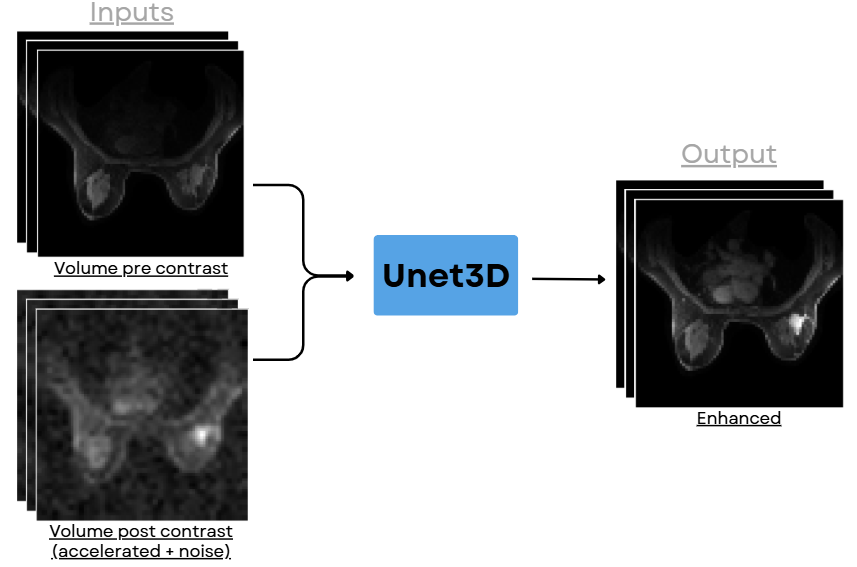
\includegraphics[width=0.75\textwidth]{image/training_pipeline.png}
    \caption{Training pipeline representation}
    \label{fig:Training_pipeline_representation}
    \vspace{0.5cm}
\end{figure}

To validate this approach, it was first necessary to build a robust training pipeline, including both data preprocessing and model training.
Once this pipeline was established, we implemented and compared several relatively simple neural network architectures. 
Finally, we developed a reliable evaluation framework to ensure that the obtained results were meaningful, reproducible, and ultimately confirm our first hypothesis.

%\subsubsection{Conception} 
\subsubsection{Datasets}
\mbox{}\\

First of all, to run our experiments and models, we worked with two different datasets:

\begin{itemize}
    \item FastMRI Breast: This dataset consists of MRI data from 300 different patients \cite{Fastmribreast}.
    The 3D breast volumes have a shape of 192 × 320 × 320 voxels, with a spatial resolution of 1.1 × 1.0 × 1.0 mm.
    The field of view (FOV) can be derived by multiplying the resolution by the image size, resulting in approximately 211 × 320 × 320 mm³.
    Each sample in the dataset includes four different time-point acquisitions.
    A time point is a moment in the dynamic sequence, and for each time point there is one 3D MRI acquisition.
    In the training pipeline, the dataset was split into two parts: 240 samples for training and 60 samples for validation, which were also used for testing.
    % Check the number o f sample in
    \item MAMA-MIA: This dataset contains MRI data from 500 different patients \cite{Mamamia}.
    The dataset contains both unilateral and bilateral breast examinations, corresponding to cases with either one or two breasts imaged.
    The 3D volume shapes vary across samples, as do the spatial resolution and the FOV.
    Each sample includes between four and six time-point acquisitions.
    The main difference compared to the other dataset is that it provides segmentation masks, highlighting the regions where the lesions are visible.
    This allows us to analyze the dynamic behavior of the contrast agent in the breast over time.
    Finally, in the training pipeline, the dataset was split into two parts: 360 samples for training and 140 samples for validation, which were also used for testing.

\end{itemize}

% GPU
\paragraph{Tools and frameworks}
\mbox{}\\
To train our models within reasonable time constraints, we relied on several GPUs with different computational capacities.
The computational resources used during the internship were the following:
\begin{itemize}
    \item \textit{Leviathan}: a server equipped with two 16~GB GPUs, mainly used for running experiments and storing the FastMRI Breast and MAMA-MIA datasets.
    \item \textit{Cthulhu}: a more powerful server with two 49~GB GPUs, dedicated to training larger and more computationally demanding models.
\end{itemize}

We extensively used GitHub throughout the internship, starting with a personal repository to safely experiment, back up our work, and learn best practices in version control such as branching, pull requests, code reviews, rebasing, issue tracking, and the use of Copilot.
Once we became comfortable with these tools, we progressively contributed directly to the company's repositories by submitting pull requests, particularly to integrate our models and training pipelines into the production codebase.

The model training was tracked online using the Weights \& Biases (W\&B) software.
It provides a code framework and interface to store and display customized content, such as the trained model weights, the evolution of metrics over the training, or even some input and output volumes for a quick visual comparison.

The most important use of W\&B in our workflow is the storage of model weights.
This is particularly useful because the trained models can be saved directly on the platform and later retrieved via the API for evaluation or testing.
Consequently, a model only needs to be trained once for a given configuration, after which it can be reused without retraining.

\subsubsection{Preprocessing}
\paragraph{Datasets}
Before developing the first training pipeline and experimenting with different model architectures, we first focused on data preprocessing.
This step involved all the necessary procedures to clean, structure, and prepare the dataset before feeding it into the training pipeline and the neural network models.

% Reshaping
\paragraph{Reshaping}
\mbox{}\\

First, it was necessary to standardize the dataset by resizing all samples to a common shape.
For example, in the FastMRI Breast dataset, each sample originally has a fixed size of 192 × 320 × 320 voxels.
Since each voxel corresponds to an input value for the model, this represents a total of 19,660,800 values per sample, which corresponds to approximately 75~MB per 3D volume.
Such a high dimensionality significantly increases both training time and GPU memory requirements.

To address this issue, we reduced the size of all samples from 192 × 320 × 320 to 64 × 80 × 80.
The in-plane resolution was reduced by a factor of 4, while the slice (through-plane) resolution was reduced by a factor of 3.
These reduction factors were chosen empirically with the main objective of decreasing computational cost rather than preserving strict physical consistency.
The downsampling was performed using a simple subsampling strategy, where, for example, a factor of 2 consists of retaining one slice out of two, without introducing any noise.

This resizing inevitably changes the spatial resolution of the data, increasing the voxel size from approximately 1.1 × 1.0 × 1.0 mm to 3.3 × 4.0 × 4.0 mm.

\begin{figure}[H]
    \centering
    \vspace{0.5cm}
    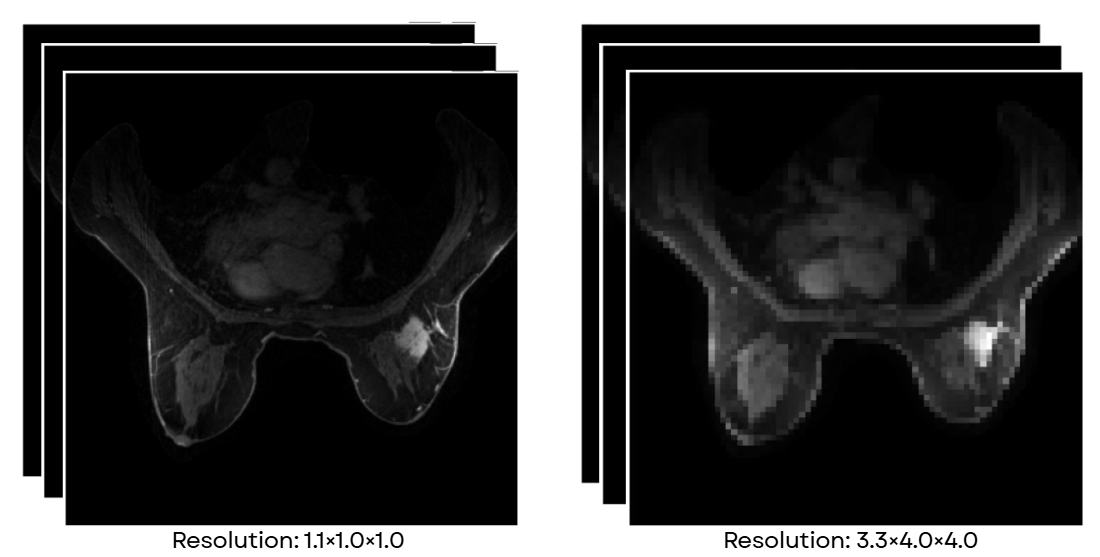
\includegraphics[width=0.75\textwidth]{image/Resolution_difference.png}
    \caption{Resolution comparison}
    \label{fig:Resolution_difference}
    \vspace{0.5cm}
\end{figure}

In the context of Chipiron, the target is to achieve a final resolution of 4.0 × 2.0 × 2.0 mm, so the final tests will be performed at this resolution.


The MAMA-MIA dataset introduces additional complexity due to variable input dimensions across samples, which required adapting the preprocessing pipeline to allow flexible resizing by directly specifying the desired output shape rather than relying on fixed per-axis configurations.

% Normalization
\paragraph{Normalization}
\mbox{}\\

Normalization is an important step in the preprocessing pipeline. It is essential to apply the same normalization method to every sample so that all inputs are represented on a comparable scale. 
Without proper scaling, activations may fall outside their optimal range, leading to poor gradient flow and reduced diversity in neuron activations, as the network first needs to compensate for scale differences before learning meaningful representations.

The most commonly used normalization method is the min-max normalization:
\[
x_{\mathrm{norm}} = \frac{x - x_{\min}}{x_{\max} - x_{\min}}
\]

However, this approach can become problematic because each sample is normalized independently.
As a result, similar tissue intensities may be mapped to very different normalized values across samples, introducing unnecessary variability in the input distribution and making the learning process less stable.

To overcome this limitation, we used percentile-based normalization:
\[
x_{\mathrm{norm}} = \frac{x - P_1(x)}{P_{99}(x) - P_1(x)}
\]

where $P_1(x)$ and $P_{99}(x)$ denote the 1st and 99th percentiles of the data distribution, respectively.

The main advantage of this method is that it reduces the influence of extreme values by ignoring the lowest 1\% and highest 1\% of the data during normalization. 
This allows the majority of the dataset to be normalized more effectively while preventing outliers from dominating the scaling process.

% undersampling
\subsubsection{Comparison of Undersampling and Downsampling}
\mbox{}\\
As explained earlier, in order to accelerate the acquisition and to capture wash-in and wash-out effects, the samples must be degraded, since this reflects the physical constraints of MRI acquisition. 
The two datasets used in this work contain fully sampled data; therefore, all samples must be artificially degraded to simulate data acquired from a low-field MRI system with accelerated acquisition.

Two main methods can be used for this purpose:

\begin{itemize}
    \item \textbf{Downsampling} is the process of reducing the number of data points in each sample of a dataset.
    In our case, it is also used as a degradation strategy to simulate low-field MRI data.
    This is achieved by increasing the downsampling factor and adding Gaussian noise.

    \item \textbf{Undersampling} is performed in the frequency domain (k-space) rather than in the spatial domain: it removes k-space samples by applying a sampling mask.
    
    k-space is a mathematical space used in MRI to represent the acquired signal in the frequency domain. 
    Each point in k-space corresponds to a specific spatial frequency component and contains complex-valued information, including both magnitude and phase. 
    It encodes the spatial information of the image by decomposing it into different frequency components, which can be transformed back into the spatial domain using an inverse Fourier transform.
    At the center of k-space are low spatial frequencies that encode global intensity and contrast; at the edges are high spatial frequencies that encode fine details and boundaries.

    Undersampling masks are used to accelerate the acquisition by not acquiring all the information in k-space.
    A mask is a binary sampling pattern applied to k-space, where a value of 1 indicates that a k-space location is acquired and a value of 0 indicates that it is omitted.
    Such masks typically preserve the center of k-space as much as possible, because it contains the most important information for reconstruction.
\end{itemize}

\paragraph{Undersampling as the retained approach}
\mbox{}\\
The undersampling strategy provides a more realistic simulation of MRI degradation because it reproduces the actual acquisition process. 
MRI scanners do not directly acquire spatial images but measure frequency-domain signals in k-space. 
Therefore, removing k-space samples through undersampling better represents accelerated or incomplete MRI acquisitions (like aliasing) compared with spatial downsampling, which mainly introduces artificial resolution loss after image reconstruction.
In this work, undersampling was therefore selected as the degradation strategy to generate realistic simulated MRI acquisitions.

\subsubsection{Generation of undersampling masks}
\mbox{}\\
To simulate different MRI acquisition schemes, three types of k-space sampling masks were considered: Cartesian, radial, and phyllotaxis-radial masks.

These masks are generated by first defining the corresponding sampling trajectories.
A trajectory describes how the MRI system samples k-space during acquisition; we then use the sampled locations as a binary mask.

The configuration can be divided into three main parts: the acquisition parameters, the readout parameters, and the trajectory parameters.
The acquisition and readout parameters are nearly identical across all trajectory types; only the trajectory parameters influence the type of mask.

\paragraph{Acquisition}
\mbox{}\\

The acquisition configuration is common to all trajectory types (\texttt{decay\_cartesian}, \texttt{stack\_of\_radial}, and \texttt{phyllotaxis\_radial}).
It is defined by three main parameters:

\begin{itemize}
    \item Field of View (FOV)
    \item Resolution
    \item Number of shots
\end{itemize}

The FOV depends on both the image resolution and the input volume size. These quantities are related by

\[
\mathrm{Resolution} = \frac{\mathrm{FOV}}{\mathrm{Input\ Shape}}.
\]

For example, in our case the input volume size is $(64, 80, 80)$ voxels and the spatial resolution is $(3.3, 4.0, 4.0)$ mm. 
The resulting FOV is therefore approximately

\[
(64 \times 3.3,\; 80 \times 4.0,\; 80 \times 4.0)
=
(211,\; 320,\; 320)\ \mathrm{mm}.
\]

Another important acquisition parameter is the number of shots. 
A sample corresponds to a single measurement point in k-space. 
A shot is a collection of samples acquired consecutively during a readout.

In our configuration, each shot contains 80 samples. 
To fully sample the k-space, 5120 shots are required. 
Therefore, the total number of acquired k-space samples is

\[
5120 \times 80 = 409\,600.
\]

For the low-field MRI system considered here, the acquisition time of a single shot is approximately 30~ms. 
Consequently, a fully sampled acquisition requires

\[
5120 \times 30 \text{ ms}
=
153.6 \text{ s}
=
2 \text{ min } 33.6 \text{ s}.
\]
To capture the dynamics of the contrast agent, multiple acquisitions must be performed over time. 
A fully sampled acquisition lasting 2~min 33.6~s is therefore too long, since the contrast agent distribution evolves continuously and important temporal information may be lost during the acquisition. 
By applying an undersampling factor of 4, the number of acquired shots is reduced from 5120 to 1280, resulting in a shorter acquisition time of 38.4~s.

\[
1280 \times 30 \text{ ms}
=
38.4 \text{ s}.
\]

\paragraph{Readout}
\mbox{}\\

The readout configuration is also common to all trajectory types.

A readout corresponds to the acquisition of a sequence of k-space samples during a single shot. 
The main readout parameter is therefore the number of samples acquired per shot.

In our experiments, each shot contains 80 samples, meaning that the readout length is fixed to 80 for all trajectory types.

\paragraph{Different sampling trajectories}
\mbox{}\\

The trajectory parameters are the only part of the configuration that varies between the different trajectory types.

They define how k-space is sampled during each shot, that is, the spatial locations of the acquired samples and the order in which they are collected.

Different trajectory models can be used, such as:

\begin{itemize}
    \item \texttt{decay\_cartesian},
    \item \texttt{stack\_of\_radial},
    \item \texttt{phyllotaxis\_radial}.
\end{itemize}

For the \texttt{decay\_cartesian} trajectory, several parameters control the sampling pattern in k-space.

The \texttt{density\_decay} parameter controls the polynomial decay used to define the sampling density distribution.
A high value of \texttt{density\_decay} results in a higher concentration of shots near the center, whereas values closer to zero lead to a more uniform distribution across k-space.

The \texttt{keep\_edges} parameter determines whether to keep the k-space edges or not, as they carry high-frequency information but not densely enough to make a significant difference.

Finally, the \texttt{sampling\_method} defines how shots are selected according to the prescribed density.
Three strategies are available: \texttt{random}, which performs stochastic sampling based on the density map; \texttt{lloyd}, which generates a pseudo-random distribution with improved spatial regularity through an iterative optimization approach; and \texttt{topk}, which uses the same spaced distribution as \texttt{lloyd} but selects only the points at the center.

\begin{figure}[H]
    \centering
    \begin{subfigure}{0.48\textwidth}
        \centering
        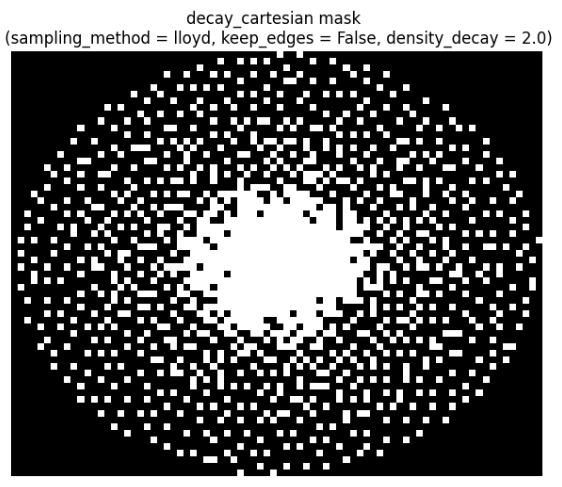
\includegraphics[width=\textwidth]{image/decay_cartesian_mask.png}
        \caption{2D slice of the Cartesian sampling mask}
        \label{fig:decay_cartesian_mask}
    \end{subfigure}
    \hfill
    \begin{subfigure}{0.48\textwidth}
        \centering
        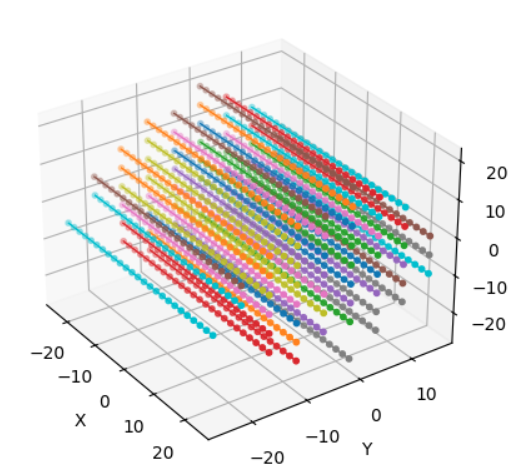
\includegraphics[width=\textwidth]{image/decay_cartesian_trajectories.png}
        \caption{3D Cartesian trajectories}
        \label{fig:decay_cartesian_trajectories}
    \end{subfigure}
    \caption{Visualization of the Cartesian sampling pattern}
    \label{fig:cartesian_sampling}
\end{figure}


For the \texttt{stack\_of\_radial} trajectory, several parameters control the sampling pattern in k-space.

The parameter \texttt{nb\_spokes} defines the number of radial spokes acquired per slice. 
It is computed from the total number of shots divided by the number of slices (or stacks). 
In our case, this corresponds to

\[
\frac{1280}{64} = 20 \ \text{spokes per slice}.
\]

The parameters \texttt{spoke\_tilt} and \texttt{stack\_tilt} control the angular distribution of the radial spokes. 
They define how successive spokes are rotated within each slice and across slices. 
These angles can follow different strategies, such as uniform spacing or a golden-angle scheme, which helps improve k-space coverage and is particularly beneficial for dynamic imaging.

\begin{figure}[H]
    \centering
    \begin{subfigure}{0.48\textwidth}
        \centering
        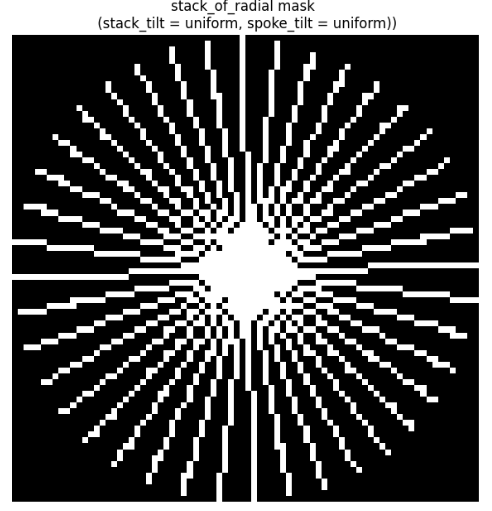
\includegraphics[width=0.75\textwidth]{image/stack_of_radial_mask.png}
        \caption{2D slice of the radial sampling mask}
        \label{fig:stack_of_radial_mask}
    \end{subfigure}
    \hfill
    \begin{subfigure}{0.48\textwidth}
        \centering
        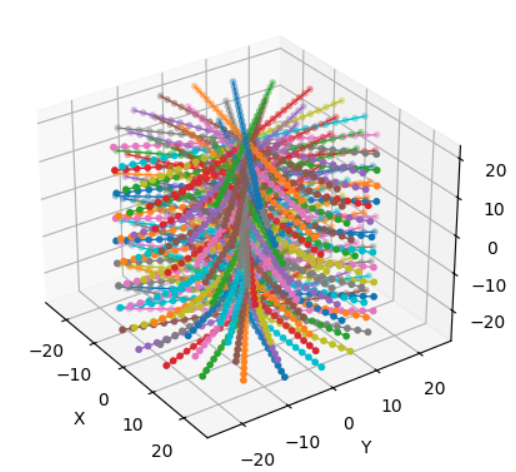
\includegraphics[width=0.75\textwidth]{image/stack_of_radial_trajectories.png}
        \caption{3D Radial trajectories}
        \label{fig:stack_of_radial_trajectories}
    \end{subfigure}
    \caption{Visualization of the radial sampling pattern}
    \label{fig:radial_sampling}
\end{figure}

Finally, the \texttt{phyllotaxis\_radial} trajectory does not introduce additional tunable parameters, as it shares the same configuration as the \texttt{stack\_of\_radial} setup.
%check what is really changing

\begin{figure}[H]
    \centering
    \vspace{0.5cm}
    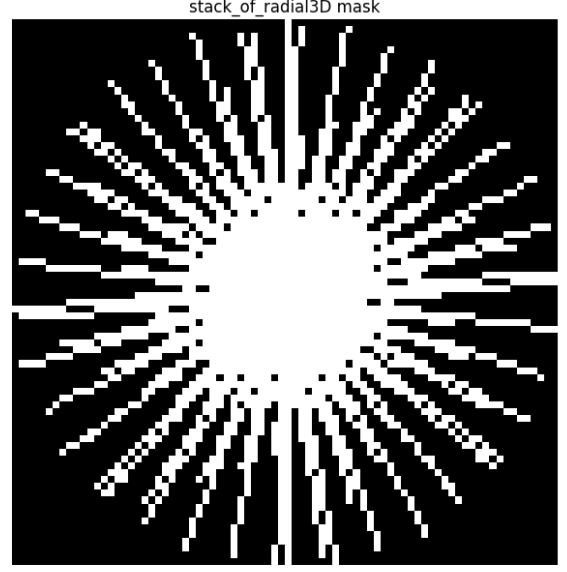
\includegraphics[width=0.75\textwidth]{image/phyllotaxis_radial_mask.png}
    \caption{2D slice of the phyllotaxis-radial sampling mask}
    \label{fig:phyllotaxis_radial_mask}
    \vspace{0.5cm}
\end{figure}

The parameters associated with the \texttt{stack\_of\_radial} and \texttt{decay\_cartesian} trajectories will be systematically explored in the third phase in order to assess their influence and identify the optimal configuration for each acquisition time.
One of the objectives of this internship is also to investigate which trajectory configuration best enhances dynamic contrast.

% Talk about the noise
\paragraph{Noise in k-space}
\mbox{}\\
Once the trajectory configurations are defined, the undersampling mask can be generated. 
However, an additional aspect must be considered: the SNR.

Since a low-field MRI system is used, the acquired signal is inherently weaker, resulting in a reduced SNR and consequently a noisier image. 
To realistically simulate this low-SNR condition, Gaussian noise is introduced during the data generation process.

In the case of undersampled acquisitions, the noise is added directly in k-space; however, only the k-space samples retained by the undersampling mask are affected by noise.
A zero-mean Gaussian distribution with a standard deviation of 200 is applied independently to both the real and imaginary components, as the data are complex-valued in the frequency domain. 
This value was empirically chosen based on multiple experiments to visually match the noise level observed in real low-field MRI acquisitions.

Furthermore, the noise can vary across k-space.
Due to the sampling density variations induced by the mask, certain regions contain more samples than others. 
For instance, in the \texttt{decay\_cartesian} trajectory, the \texttt{density\_decay} parameter leads to a higher concentration of samples in the center of k-space. 
In these regions, the effective noise level should be lower due to increased redundancy of information.

To account for this effect, the noise amplitude is scaled by the inverse square root of the local sampling density. 
This follows the assumption that regions with higher sampling density benefit from noise averaging, resulting in lower noise variance.
The local noise standard deviation is therefore defined as:
\[
\sigma(k)=\frac{\sigma_0}{\sqrt{\rho(k)}}
\]

where $\sigma_0$ is the reference noise level and $\rho(k)$ is the local sampling density.
This ensures that regions with higher sampling density exhibit a reduced noise variance, making the simulated k-space more consistent with realistic low-field MRI acquisition physics.

Figures~\ref{fig:decay_cartesian_example}, \ref{fig:stack_of_radial_example} and \ref{fig:phyllotaxis_example} show examples of the resulting images, with the undersampling and the noise added depending on the mask used.

\begin{figure}[H]
    \centering
    \vspace{0.5cm}
    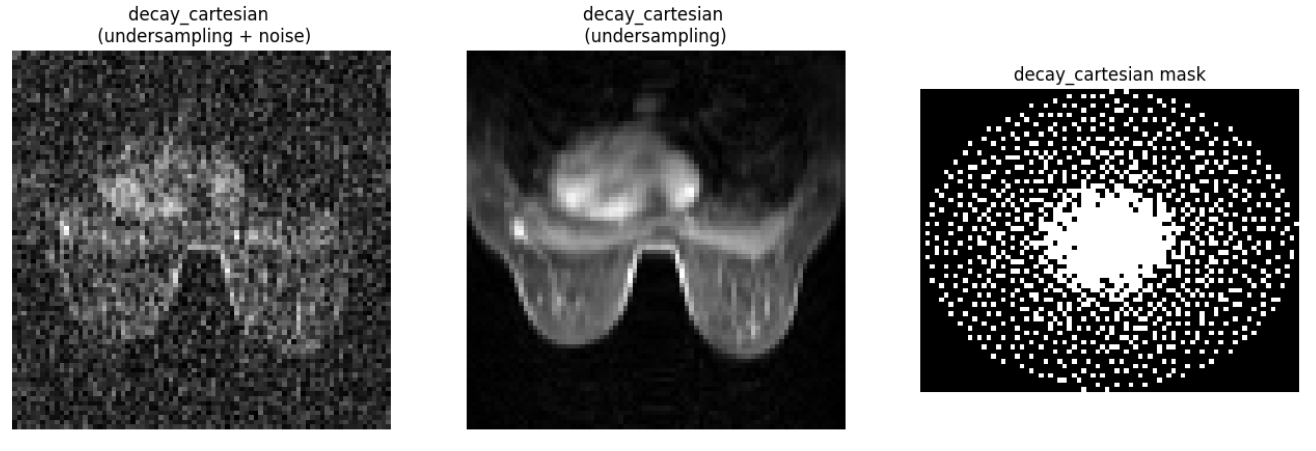
\includegraphics[width=0.75\textwidth]{image/decay_cartesian_example.png}
    \caption{Undersampled \texttt{decay\_cartesian} images with and without noise}
    \label{fig:decay_cartesian_example}
    \vspace{0.5cm}
\end{figure}

\begin{figure}[H]
    \centering
    \vspace{0.5cm}
    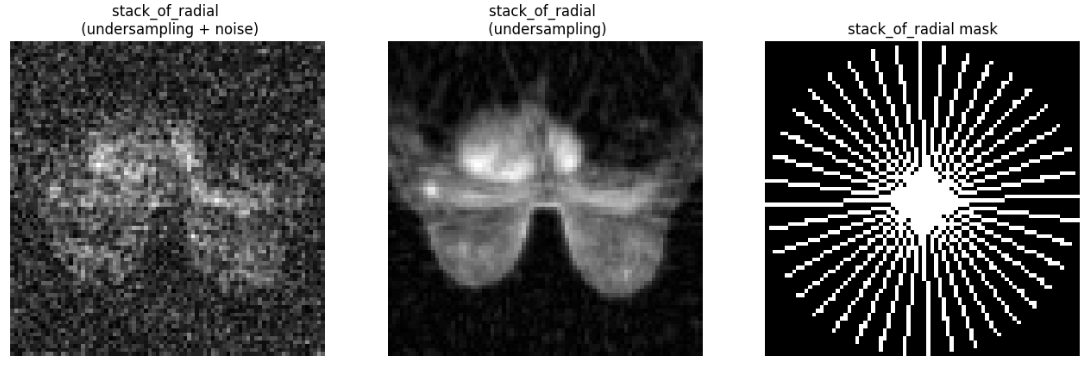
\includegraphics[width=0.75\textwidth]{image/stack_of_radial_example.png}
    \caption{Undersampled \texttt{stack\_of\_radial} images with and without noise}
    \label{fig:stack_of_radial_example}
    \vspace{0.5cm}
\end{figure}

\begin{figure}[H]
    \centering
    \vspace{0.5cm}
    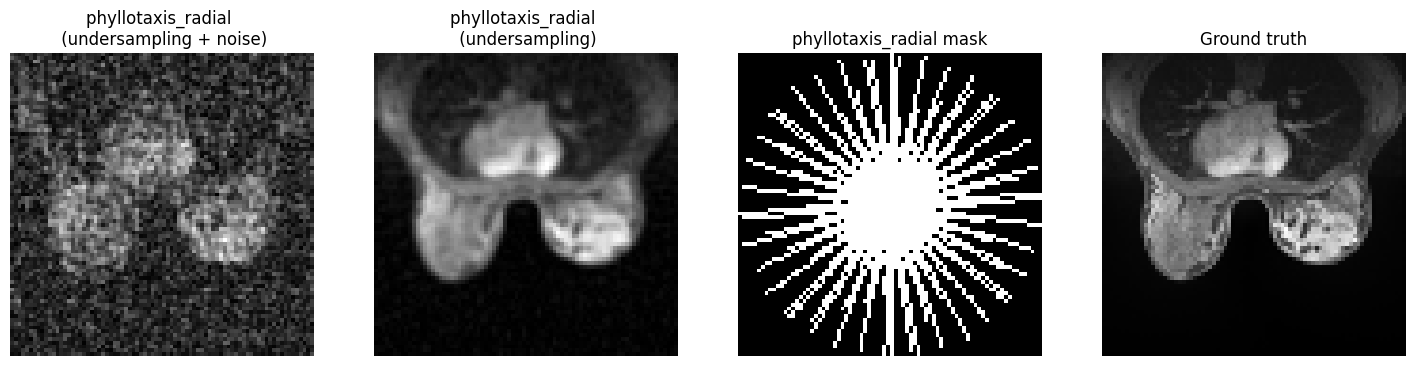
\includegraphics[width=0.75\textwidth]{image/phyllotaxis_radial_example.png}
    \caption{Undersampled \texttt{phyllotaxis\_radial} images with and without noise}
    \label{fig:phyllotaxis_example}
    \vspace{0.5cm}
\end{figure}


\subsubsection{Training pipeline}


Now that the preprocessing stage has been completed and realistic low-field MRI data have been generated, including accelerated acquisitions obtained through undersampling techniques, the next step is to establish the training pipeline for the deep learning models.

Rather than being independent components, the different stages of the pipeline operate sequentially, with the output of one stage serving as the input to the next. 
The complete training pipeline is organized into five main components:

\begin{itemize}
    \item The preprocessing script, which prepares the high-resolution MRI data before training.
    \item The data loading pipeline, responsible for generating the noisy low-field images and feeding the data to the model.
    \item The neural network, which defines the model architecture and contains the trainable parameters optimized during the learning process.
    \item The training script, which defines the training procedure, including the loss function, backpropagation, epochs, batch size, and early stopping (patience).
    \item The main script, which orchestrates the entire workflow by executing each stage in the correct order.
\end{itemize}

The following sections describe each component in detail and explain how they are combined into a complete training pipeline.

\paragraph{Preprocessing script}
\mbox{}\\


First of all, before launching the training pipeline, a preprocessing script can be used to reduce the image resolution and ensure that all samples have
a consistent size as explained earlier. The processed data are saved in a separate folder, allowing the training pipeline to directly use these lower-resolution samples.
This reduces computational cost and speeds up the training process as explained above.


During preprocessing, two segmentation masks are also saved with the new dataset. The first mask is designed to keep only
the relevant region of each sample. In many acquisitions, large areas surrounding the object of interest contain only black pixels,
which do not carry any useful information. Keeping these empty regions could negatively influence the model during the training, as it may learn to denoise
or reconstruct irrelevant background areas instead of focusing on meaningful structures.


\begin{figure}[H]
    \centering
    \vspace{0.5cm}
    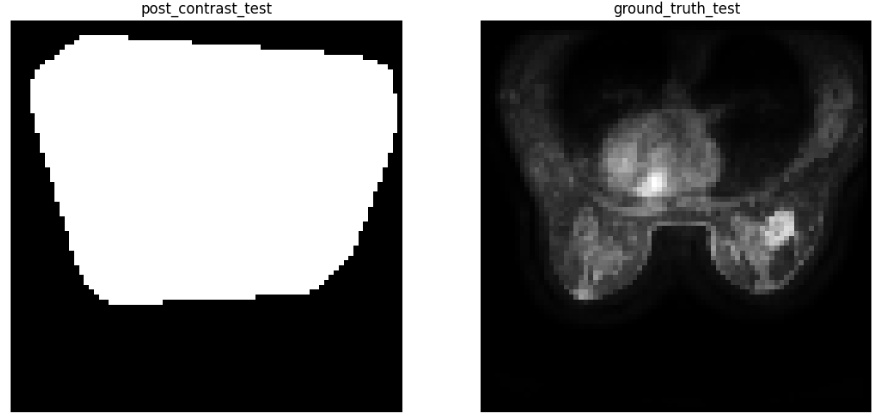
\includegraphics[width=0.75\textwidth]{image/mask_ground_truth.png}
    \caption{Mask Ground truth}
    \label{fig:mask_ground_truth}
    \vspace{0.5cm}
\end{figure}


The second mask is only available in the MAMA-MIA dataset and is not provided in the FastMRI Breast dataset. This segmentation mask specifically
identifies breast cancer lesions, allowing us to know where the contrast agent is expected to appear within the breast lesion tissue.
The segmentation masks were initially generated automatically using a segmentation network and subsequently reviewed and corrected by multiple experts, resulting in highly accurate annotations~\cite{Mamamia}.


This mask is essential for studying the contrast dynamics, as it enables the analysis to focus exclusively on the enhanced regions rather
than the entire breast. Additionally, it can be used in the training process to guide the model's attention toward contrast
areas, which are often the most clinically relevant features, instead of treating all regions of the sample equally.


\begin{figure}[H]
    \centering
    \vspace{0.5cm}
    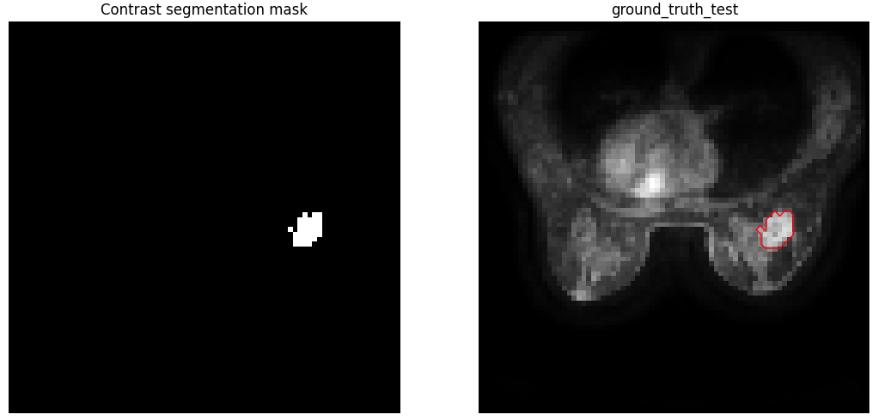
\includegraphics[width=0.75\textwidth]{image/segmentation_contrast_mask.png}
    \caption{Segmentation contrast mask}
    \label{fig:segmentation_contrast_mask}
    \vspace{0.5cm}
\end{figure}

The preprocessing script ensures that all images have the same spatial resolution and that the two corresponding segmentation masks are loaded for each sample. 
It is applied to both the training and the test datasets. 
At this stage, however, no noise has been added to the images. 
The generation of noisy low-field MRI data is performed later by the data preparation class.

\paragraph{Dataset Loading and Preparation Class}
\mbox{}\\
After running the preprocessing script, a dedicated class named \texttt{LoadingFastMRIBreastDataset3D} is used to ensure that the dataset is properly organized before being fed into the model.


First, the class loads the data from the directory containing the \texttt{.h5} files. It then separates the different acquisitions for each patient, as each
sample contains between four and six acquisitions. For every subject, the first acquisition is considered as the pre-contrast image. As for the post-contrast images,
either all available acquisitions can be included in the training set, or a single one can be randomly selected, depending on the chosen strategy.
Initially, we selected one acquisition randomly.


A corresponding ground truth is also defined, which corresponds to the same post-contrast acquisition without any acceleration applied.
This allows a direct comparison between accelerated and fully sampled data, so that the model can learn and adjust based on the ground truth.
This is described in more detail in the training section.


Next, each volume is normalized using a percentile-based normalization method, as described previously.
Finally, only the post-contrast volumes are subjected to an undersampling operation in order to simulate the effects of accelerated low-field MRI acquisitions,
while the pre-contrast and ground truth images remain fully sampled.


Moreover, the dataset also provides two segmentation masks for each sample, as previously introduced. A final important piece of information is the acquisition timestamps.
These timestamps are available for all acquisitions in the dataset and indicate the exact acquisition time of each MRI scan.


The timestamps of each acquisition represent how long it took the MRI device to perform the acquisition.
They are quite important for us because, by having the timestamps, we can easily separate the acquisitions in the testing phase and observe the dynamics of the contrast over time.


At the end, this class can return the pre-contrast images, the accelerated post-contrast images, the ground truth, the two segmentation masks, and the timestamps.
Depending on the configuration, it is possible to choose which elements are returned.


However, the three main outputs will always be returned: the pre-contrast images, the accelerated post-contrast images, and the corresponding ground
truth. In the case of the FastMRI Breast dataset, the contrast segmentation mask is not available, so the pipeline is designed to handle this situation and
avoid requiring it.


For datasets where both segmentation masks are available, they can optionally be used, as they may improve performance.
Nevertheless, the model can also be trained without them, which makes it possible to compare results with and without the use of segmentation information.

This part ensures that the input data are properly prepared before being fed into the network. 
The next step is to introduce the neural network architecture and explain how its parameters are optimized during the training process.

\paragraph{Introduction to artificial neural networks}
\mbox{}\\

The neural network is the core component of the training pipeline. 
It receives the pre-contrast and accelerated post-contrast acquisitions as inputs and aims to reconstruct the corresponding high-quality post-contrast image. 
Its architecture defines how information is processed through the different layers, while its trainable parameters (weights and biases) are optimized during training.

\paragraph{Training script}
\mbox{}\\

The training script is important because it directly affects how the model learns. In deep learning, the dataset is typically split into a
training set and a validation set. The training set is used to optimize the model, while the validation set is used during training to monitor
performance and tune hyperparameters. Unlike the validation set, the test set is only used at the end to evaluate the model on unseen data.

\paragraph{Monitoring Training}
\mbox{}\\

We need both a training dataset and a validation dataset to ensure that the model does not overfit. Overfitting occurs when a model performs very
well on the data it was trained on but poorly on new, unseen data. Therefore, using separate datasets is essential to assess the model's ability
to generalize.

During training, several important parameters in deep learning must also be carefully considered and understood.

\paragraph{Batch size}
\mbox{}\\

The first important parameter is the batch size, which represents the number of samples processed simultaneously during training. In general,
larger batch sizes can speed up training because more samples are handled in parallel. For example, training with a batch size of 8 is logically
faster than with a batch size of 4.


However, larger batch sizes also require more GPU memory, especially when dealing with large volumetric data containing many voxels. In our case,
we chose a batch size of 4 because it provided a good balance between training speed and the available GPU memory.


When the model is trained at full image resolution at the end of the internship, the batch size will likely need to be reduced
to 1 due to the large size of each sample.


\paragraph{Loss}
\mbox{}\\
The loss function measures the error between the outputs generated by the model and the ground truth target images. It plays a crucial role during
training, as the objective is to minimize this error over time.

Two of the most commonly used loss functions are the Mean Squared Error (MSE) and the Mean Absolute Error (MAE). The MSE computes the average squared
difference between the predicted outputs and the ground truth, whereas the MAE computes the average absolute difference. The main difference between
them is that the MSE is more sensitive to outliers because larger errors are penalized more heavily.


It is also possible to combine these two loss functions. In our case, we chose the MSE because we did not expect a significant number of outliers in the data.


\paragraph{Gradient descent}
\mbox{}\\
Gradient descent is an important optimization method used to minimize the cost function, in our case the loss, by progressively adjusting the model parameters, which are
mainly the weights and biases.

It is based on computing the partial derivatives of the loss with respect to these parameters. Another key element is the learning rate,
which controls the size of each update step during optimization. If the learning rate is too high, the algorithm may fail to converge to the minimum, so
it must be carefully tuned. We chose a learning rate of $10^{-4}$, which slows down the training slightly but allows the cost function to converge reliably.

\paragraph{Backpropagation}
\mbox{}\\

Backpropagation works together with gradient descent. It computes the gradient of the loss function layer by layer, starting from the output layer and moving
backward through the network. Once all gradients are computed, gradient descent uses them to update the weights and biases.

In other words, backpropagation calculates how each parameter contributes to the error, and gradient descent applies these values to adjust the model
parameters.


\paragraph{Epoch}
\mbox{}\\


An epoch represents each time all the samples from our dataset have gone through the model. At the end of each epoch, the average training loss and validation loss are computed.
The goal is to check the model's learning progress by observing how these losses evolve over time, using the W\&B software introduced earlier, where training and
validation loss curves are plotted across epochs.


\paragraph{Patience}
\mbox{}\\


Finally, another important parameter during training is the patience. Patience refers to the number of consecutive epochs during which we allow the
validation loss to not improve before stopping the training.


During training, we compute two losses: the training loss and the validation loss. The training loss is used to update the model parameters through
backpropagation and gradient descent. In contrast, the validation loss is not used for updates; it is only used to evaluate how well the model generalizes
and to detect overfitting.


Patience is applied only to the validation loss. It helps detect overfitting during training. For example, with a patience of 10, if the validation loss
does not improve for 10 consecutive epochs while the training loss continues to decrease, it indicates that the model is starting to overfit the training
data.


In that case, continuing the training is not useful, since the model is no longer improving its ability to generalize to unseen data.
This part describes how deep learning is performed using a neural network and a training script. 
All these different components are then integrated and managed through the main script, which controls the entire training pipeline.


\paragraph{Main script}
\mbox{}\\

The main script controls the entire training pipeline. It manages the preprocessing script, the \texttt{LoadingFastMRIBreastDataset3D} class, as well as all the training steps described above.
It also saves the model on W\&B and evaluates it using different metrics that will be explained later. To start the training, we run this main script,
which centralizes everything. It also allows us to choose different configurations for both the model and the training pipeline.


We created several YAML configuration files to easily change settings. Depending on the chosen configuration, we can test different options such as downsampling,
undersampling, or the use of segmentation masks. There is also a default configuration, which is the simplest setup. This allows anyone to run the pipeline directly
or modify the YAML files to experiment with different settings. This YAML-based setup is very useful because it allows us to test different configurations
easily and to identify which one gives the best results.


\subsubsection{Model architectures}
\paragraph{Artificial neural network}
\mbox{}\\

Now that the entire training pipeline was operational, a first deep learning network could be tested to determine whether its performance was sufficient to validate our first hypothesis.

Neural networks consist of an input layer, multiple hidden layers, and an output layer, whose structure depends on the desired prediction.
Each hidden layer is composed of numerous parameters, called weights, which are numerical values that define the strength of the connections between neurons.

During training, the network learns by adjusting these weights through a process involving forward propagation and backward propagation.
Forward propagation computes the model's predictions, while backward propagation updates the weights based on the prediction errors to improve the network's performance over time.

A neural network is composed of several important components, such as convolutional layers, activation functions, normalization layers, and max pooling, that need to be understood before discussing a specific architecture.

\paragraph{Convolutional neural network (CNN)}
\mbox{}\\

A Convolutional Neural Network (CNN) is a specialized type of deep learning architecture designed for tasks involving image analysis and recognition, which makes it particularly well suited to our problem.
CNNs are highly effective at identifying patterns and extracting relevant features from images, such as edges, textures, and shapes.
They are composed of several layers, each applying multiple learnable filters to the input image and producing a set of output channels.
These filters can have dimensions such as 3 × 3 × 3 or 5 × 5 × 5 in the case of three-dimensional images, and their weights are optimized during training to detect different types of features within the images.
As the input passes through the network, each filter generates a feature map that highlights the presence and spatial location of specific patterns.
By combining information extracted at different layers, CNNs progressively learn complex and abstract representations of the input image.


\paragraph{Activation function}
\mbox{}\\

Activation functions are fundamental components of neural networks, as they introduce non-linearity into the model and allow it to learn complex relationships within the data. 
Without activation functions, a neural network would behave as a simple linear model, regardless of its number of layers.

In most architectures, the activation function is applied after each convolutional operation. 
It transforms the output feature maps by applying a non-linear function before passing the information to the following layer.

Several activation functions can be used depending on the application. 
One of the most commonly used functions is the Rectified Linear Unit (ReLU), which replaces all negative values with zero while keeping positive values unchanged. 
Another commonly used function is the sigmoid activation, which maps input values into a range between 0 and 1.


\paragraph{Batch Normalization vs Instance Normalization}
\mbox{}\\


Training deep neural networks is complicated by the fact that the distribution of each layer's input changes during training as the parameters of the previous layers change.
This slows down training by requiring lower learning rates and careful parameter initialization, and it makes it hard to train models with saturating nonlinearities.
This phenomenon is known as internal covariate shift and can be mitigated by normalizing the pre-activation layers.
The goal is to make normalization part of the model's architecture; two different approaches are commonly used:


\begin{itemize}
    \item Batch Normalization (BN): it normalizes each feature map by computing the mean and the variance over all the examples in the batch.
    It has two learnable parameters: $\gamma$ for the scaling and $\beta$ for the shifting.
    The parameter $\beta$ can replace the bias that we have in the feature map. % Formula ?
    \[
    \hat{x}_i = \frac{x_i - \mu_B}{\sqrt{\sigma_B^2 + \epsilon}}
    \]


    \[
    y_i = \gamma \hat{x}_i + \beta
    \]


    Knowing that $\mu_B$ represents the mean of the batch and $\sigma_B^2$ the variance of the batch, $\epsilon$ is a small constant added to avoid division by zero.
    Finally, $\gamma$ and $\beta$ are learnable parameters of the model.


    \item Instance Normalization (IN): it normalizes each feature map by computing the mean and the variance separately for every feature map across its spatial dimensions.
    It also has two learnable parameters, as in BN. % Formula ?
    \[
    \hat{x}_{h,w,d} = \frac{x_{h,w,d} - \mu_I}{\sqrt{\sigma_I^2 + \epsilon}}
    \]
    \[
    y_{h,w,d} = \gamma \hat{x}_{h,w,d} + \beta
    \]
    The only change is that $\mu_I$ represents the mean of the sample and $\sigma_I^2$ the variance of the sample, not of the batch.


\end{itemize}


Batch Normalization significantly improves training stability by reducing internal covariate shift and accelerates convergence.
It stabilizes learning by making the model's activations more consistent across different batches and ensures faster convergence, allowing the use of larger learning rates.
Instance Normalization, on the other hand, does not directly improve training speed or stability, but it allows models with large inputs (e.g., medical images) to be trained with small batch sizes.
This is often required by hardware limitations (GPU size).


\paragraph{Max pooling}
\mbox{}\\


Max pooling is an operation typically used in CNNs because it reduces the spatial dimensions by sliding a 3D window and taking the maximum value in each region.
It performs downsampling and reduces computation while retaining the most important features.

Most deep learning models rely on core components such as convolutional layers, activation functions, batch normalization, and max pooling, which are essential for building stable neural networks, particularly in medical imaging applications.
However, the main differences lie in the network architecture, which can vary considerably depending on the specific problem.
In this work, we experimented with several architectures, which will be presented in the following section.


\paragraph{NoNew-Net}
\mbox{}\\
The first architecture we investigated to validate the first hypothesis was NoNew-Net \cite{NoNewNet}, which is based on a U-Net architecture.
U-Net architectures are widely used in deep learning and have served as the foundation for numerous successful models in medical image analysis, particularly for segmentation tasks.
In our application, U-Net architectures have also demonstrated strong performance for image denoising while remaining relatively simple to implement.
The main argument of NoNew-Net is that the architecture outperforms more complicated ones without unnecessarily complex layers \cite{NoNewNet}.
For these reasons, NoNew-Net was selected as a baseline model for our experiments.


NoNew-Net is organized into several blocks, each corresponding to a different resolution level.
It follows the classical encoder-decoder structure of a U-Net with skip connections.
At each stage of the encoder, the spatial dimensions of the feature maps are reduced by a factor of two using max pooling, while the number of feature channels is typically doubled to extract higher-level features.
In the decoder, the feature maps are progressively upsampled, increasing their spatial dimensions by a factor of two at each stage, while the number of feature channels is reduced accordingly.
Finally, skip connections are used to transfer information from the encoder to the corresponding decoder levels, allowing the network to preserve fine spatial details during the reconstruction process.


For each architecture, a configuration file in YAML format was used, as for the training pipeline introduced earlier.
The NoNew-Net architecture uses a kernel size of 3, corresponding to a 3D convolutional filter of size 3 × 3 × 3.
The base number of feature channels is set to 30 and is progressively increased throughout the encoder, typically doubling at each block.
The number of blocks was set to 4; as a result, the block at the bottom of the U-Net, which we call the bottleneck layer, contains 480 feature channels.
The activation function used is Leaky ReLU. Unlike standard ReLU, it introduces a small negative slope (0.2), meaning that negative values are not entirely set to zero but are instead scaled down.
Finally, an important design aspect of the model concerns the number of input and output channels, which depends most of the time on the specific problem being addressed.
In our case, the model takes two input channels corresponding to pre-contrast and post-contrast acquisitions.
These two inputs are concatenated along the channel dimension to form a single tensor with two channels.
This is why the model is configured to start with 2 input channels.


\[
X = \mathrm{Concat}(X_1, X_2)
\]


\[
X_1, X_2 \in \mathbb{R}^{B \times 1 \times D \times H \times W}
\]


\[
X \in \mathbb{R}^{B \times 2 \times D \times H \times W}.
\]


As for the output, we only want one channel, because the ground truth has one channel and we need the same dimensions to compute the cost function (loss).

\subsubsection{Experiments}

The objective of the evaluation is to assess the performance of the NoNew-Net model to validate our first hypothesis.

As explained previously, to evaluate whether the neural network is able to enhance post-contrast acquisitions based on fully sampled pre-contrast and accelerated noisy post-contrast inputs, its performance is assessed according to two main objectives:
\begin{itemize}
    \item Reconstruct high-quality images from noisy and undersampled MRI acquisitions over time.
    \item Enhance the image contrast throughout the temporal sequence.
\end{itemize}

The evaluation was performed using both qualitative and quantitative approaches. 
The qualitative assessment relied on visual inspection of the reconstructed images to evaluate the preservation of anatomical structures and contrast enhancement. 
The quantitative assessment was based on objective image quality metrics to measure reconstruction accuracy.

For each experiment, three evaluation metrics are used:

\begin{itemize}
    \item \textbf{RMSE (Root Mean Square Error):} This metric measures the voxel-wise difference between the reconstructed image and the reference image. 
    An RMSE value close to 0 indicates a high similarity between the two images, whereas larger values correspond to greater reconstruction errors.
    
    \item \textbf{PSNR (Peak Signal-to-Noise Ratio):} PSNR is derived from the RMSE and expresses the reconstruction quality on a logarithmic scale. 
    Unlike RMSE, higher PSNR values indicate better reconstruction quality. 
    Values around 40~dB or higher generally correspond to very similar images.
    
    \item \textbf{SSIM (Structural Similarity Index Measure):} Unlike RMSE and PSNR, SSIM evaluates the structural similarity between two images by comparing luminance, contrast, and structural information rather than individual voxels. 
    A value close to 1 indicates a high structural similarity, while values closer to 0 indicate poor agreement.
\end{itemize}

\paragraph{Full-Sample Evaluation}
\mbox{}\\

The first evaluation consists of a qualitative and quantitative analysis of each sample coming out of the network. 
Indeed, one of the most effective ways to assess the performance of a neural network is to visually compare its output with the corresponding ground truth.

For each test, four images are displayed:
\begin{itemize}
    \item The \textbf{pre-contrast input}, which is a fully sampled acquisition without undersampling or additional noise.
    It provides a high-quality reference of the anatomical structures.
    \item The \textbf{post-contrast input}, which has been undersampled and corrupted with noise to simulate the acquisition of a low-field MRI scanner.
    \item The \textbf{model output}, corresponding to the image reconstructed by the neural network.
    \item The \textbf{ground truth}, which serves as the reference image. 
    The objective is for the reconstructed image to be as close as possible to this reference.
\end{itemize}

The first step of the evaluation is a visual inspection to determine whether the network successfully reconstructs the missing information and produces an image that resembles the ground truth while improving upon the input image.

To complement the visual analysis, the three metrics introduced in the previous section (RMSE, PSNR, and SSIM) are computed between the model output and the ground truth. 
They are also computed between the input images (post-contrast and pre-contrast) and the ground truth. 
This comparison is essential to verify that the network effectively improves the image quality. 
If the reconstructed image does not achieve better metric values than the input images, it indicates that the network has failed to learn the desired mapping and may even degrade the image quality.

The second row of the figure displays the absolute difference between each image and the ground truth. 
These error maps highlight the regions where the reconstruction differs the most from the reference image, allowing us to identify the anatomical structures that remain difficult for the network to reconstruct. 
A color bar is used to facilitate the interpretation of the error magnitude.

Finally, the third row presents the signed difference between each image and the ground truth. 
Unlike the previous row, the absolute value is not applied, making it possible to distinguish overestimation from underestimation. 
Red regions indicate voxel intensities that are higher than the ground truth, blue regions correspond to lower intensities, and white regions represent negligible differences, indicating an accurate reconstruction.

\begin{figure}[H]
    \centering
    \vspace{0.5cm}
    
\includegraphics[width=0.75\textwidth]{\detokenize{image/Full sample qualitative evaluation.png}}
    \caption{Full sample qualitative evaluation}
    \label{fig:full_sample_qualitative_evaluation}
    \vspace{0.5cm}
\end{figure}

In this example, the output images are visually very close to the ground truth, both in appearance and in terms of the metrics compared to the input. 
This test shows that, for this sample, the network is able to reconstruct the volume very accurately.

%explanation of result

\paragraph{Contrast Evaluation}
\mbox{}\\

To evaluate the contrast enhancement, RMSE, PSNR, and SSIM are not suitable because the contrast agent is confined to a relatively small segmented region. 
These metrics are very efficient to compare the entire sample but they do not accurately reflect the quality of the contrast reconstruction.

Instead, the temporal evolution of the contrast intensity is analyzed.
For each sample, the mean intensity within the segmented contrast region only is computed for every acquisition.
The resulting intensity curves are then plotted for both the model output and the ground truth.

The objective is for the reconstructed intensity curve to closely follow the ground-truth curve. 
A good match indicates that the network not only enhances the contrast but also correctly reproduces its temporal dynamics. 
This is particularly important because the model should not generate a constant level of contrast enhancement across all acquisitions. 
Instead, it must preserve the physiological evolution of the contrast agent over time, including both the wash-in and wash-out phases.

\begin{figure}[H]
    \centering
    \vspace{0.5cm}
    
\includegraphics[width=0.75\textwidth]{\detokenize{image/Dynamic contrast intensity.png}}
    \caption{Dynamic contrast intensity}
    \label{fig:dynamic_contrast_intensity}
    \vspace{0.5cm}
\end{figure}

\begin{figure}[H]
    \centering
    \vspace{0.5cm}
    
\includegraphics[width=0.75\textwidth]{\detokenize{image/Full sample contrast dynamic.png}}
    \caption{Full sample contrast dynamic}
    \label{fig:full_sample_contrast_dynamic}
    \vspace{0.5cm}
\end{figure}


In this example, three curves are shown. 
The red curve represents the mean intensity of each segmentation for each network input acquisition of one patient.
The blue curve represents the mean intensity of the network output after contrast reconstruction, while the black curve corresponds to the original contrast mean intensity.

The second plot illustrates the evolution of the contrast for each sample.
The first row shows the input of the network, with the pre-contrast acquisition and all the post-contrast acquisitions.
The second row shows the output of the network, with the post-contrast acquisitions that have been enhanced.
The last row shows the ground truth for each acquisition.
Finally, in this visualization, the red regions correspond to the segmented areas for each acquisition, where we compute the mean intensity of the three curves.

For this sample, the model appears to accurately reproduce the contrast enhancement, as the predicted intensity distribution closely matches the ground truth.

\subsubsection{Conclusion} 

In this first phase, we developed a fully operational training pipeline with a robust data preprocessing workflow.
We also implemented one network architecture that can be trained and evaluated within the same framework.
Finally, we established a comprehensive evaluation strategy to verify that a simple network is able to reconstruct both the entire volume and the contrast enhancement.

The results demonstrate that the network is able to enhance the contrast using a fully sampled pre-contrast acquisition and an accelerated post-contrast acquisition as inputs. 
The obtained metrics show promising performance, supporting the validation of the first hypothesis.

In the second phase, we will focus on testing different deep learning networks with a more accurate representation of the pre-contrast and post-contrast inputs for our fast-acquisition low-field MRI application.


\subsection{Transition to Realistic Acquisition Conditions} 

\subsubsection{Methodology} 

The first phase of this work focused on developing a robust training pipeline and a reliable evaluation framework to demonstrate that deep learning models were capable of enhancing post-contrast images by exploiting both pre-contrast and post-contrast information.
The objective of the second phase is to compare different deep learning networks on a more realistic reconstruction task by generating input data that better reflect the characteristics of low-field MRI acquisitions.

In the initial pipeline, the network received two inputs: a pre-contrast image, fully sampled without noise, and a post-contrast image, undersampled and corrupted with noise to simulate a low-field MRI acquisition. 
While this setup allowed the models to learn the reconstruction task, it did not accurately represent real acquisition conditions. 
In practice, even a pre-contrast scan acquired on a low-field MRI system contains measurement noise.
Moreover, it is inconvenient for the patient to first undergo a full pre-contrast acquisition and to later undergo multiple additional post-contrast acquisitions.

To better reproduce these conditions, we generated a single long acquisition spanning the pre-contrast and post-contrast phases.
We then compute its average, which is used as the network input.
Because this averaged acquisition combines multiple shots, it has a higher SNR and is therefore less noisy than any individual acquisition.
This mean long acquisition is then used as the network input to enhance each noisy fast acquisition independently throughout the dynamic sequence.
This modification significantly increased the difficulty of the reconstruction problem.

\begin{figure}[H]
    \centering
    \vspace{0.5cm}
    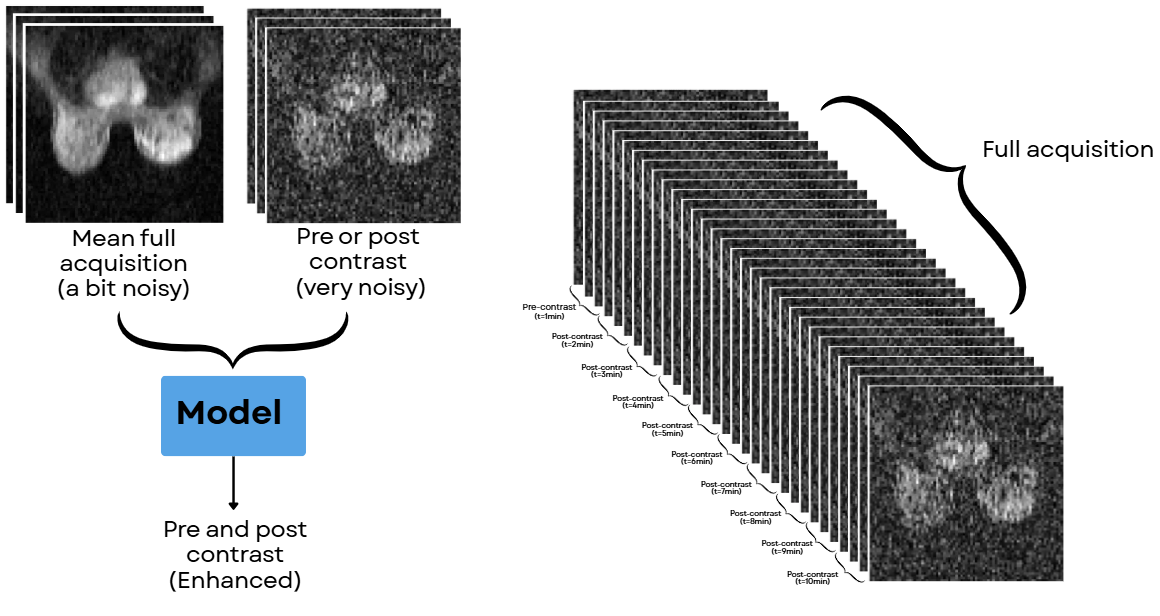
\includegraphics[width=0.75\textwidth]{image/Training pipeline full acquisition.png}
    \caption{Training pipeline full acquisition}
    \label{fig:Training pipeline full acquisition}
    \vspace{0.5cm}
\end{figure}


Once this new acquisition paradigm had been established, the study was extended beyond the initial NoNew-Net architecture. 
Several deep learning models were implemented and compared using a quantitative evaluation framework in order to identify the architecture best suited to this reconstruction task.

The main objective of this second phase was therefore to identify the deep learning architecture that provides the best trade-off between reconstruction quality and robustness under strong realistic low-field MRI acquisition conditions.

\subsubsection{Modification of Training pipeline} 

First of all, as explained in the methodology, we need to have a full-sample acquisition and to compute its average to use as the input.
Instead of acquiring a single pre-contrast image, we consider a full 10-minute acquisition divided into ten shorter acquisitions. 
These acquisitions are then averaged to produce a noisy full acquisition sample. 
Averaging multiple acquisitions increases the SNR by exploiting all the available information while preserving the anatomical structures. 
This averaged image is subsequently used as full acquisition image input for reconstructing the pre-contrast and each individual post-contrast acquisition.

However, in the available dataset, only one pre-contrast image and between three to five post-contrast acquisitions are available rather than ten acquisitions. 
To reproduce the proposed acquisition strategy, a weighted average is computed by completing the missing acquisitions with the pre-contrast image. 
This assumption is physiologically reasonable since, once the contrast agent has completely washed out, additional acquisitions would become equivalent to pre-contrast images.

The resulting averaged full-acquisition image is then undersampled using the same sampling mask as the pre-contrast and post-contrast acquisitions.
To account for the longer effective acquisition time, the noise level is reduced by a factor of $\sqrt{10}$. 
The factor is $\sqrt{10}$ because we are assuming that each acquisition is 1 minute.
This follows the well-known relationship between acquisition time and SNR in MRI: averaging $N$ independent acquisitions increases the SNR by a factor of $\sqrt{N}$. 
Consequently, using the equivalent of ten acquisitions produces a cleaner and more realistic input image while remaining consistent with the physics of MRI acquisition.

\subsubsection{Architecture models}

In the first phase, the NoNew-Net architecture demonstrated that it was possible to successfully enhance post-contrast images by using two input acquisitions.
In the second phase, with a full-sample acquisition replacing the pre-contrast input, the objective was to investigate alternative neural network architectures and determine which one is the most effective for our new reconstruction task.

\paragraph{NoNew-Netv2}
\mbox{}\\
The main difference between NoNew-Net and NoNew-Netv2 is in the decoder, more specifically in the upsampling strategy.
In the original NoNew-Net, the feature maps are upsampled using an interpolation function.
This operation does not involve any learnable parameters; it simply increases the spatial resolution by applying a mathematical interpolation.
After this step, a normal convolution, as in the encoder, is applied to learn how to combine and refine the features in the decoder.

In NoNew-Netv2, the interpolation layer is replaced by a 3D transposed convolution (ConvTranspose3D).
Unlike interpolation, a transposed convolution contains learnable parameters that are optimized during training.
As a result, it not only upsamples the feature maps but also learns the upsampling operation itself.

The advantage of interpolation is that it is computationally cheaper and does not introduce additional parameters, making it faster and more memory-efficient.
In contrast, transposed convolution increases the number of trainable parameters and the computational cost.
It also provides greater flexibility by learning a better upsampling adapted to our specific task, which can improve the reconstruction of samples.

% architecture example
\paragraph{ResU-Net}
\mbox{}\\


The second architecture we investigated was a residual version of the U-Net.
Instead of directly predicting the post-contrast image, the network predicts the residual which is the difference between the pre-contrast and post-contrast acquisitions.


The intuition behind this approach is that the anatomical structures are already present in the pre-contrast image, while the contrast agent only modifies a limited number of regions.
Consequently, learning the residual is an easier task than reconstructing the entire post-contrast image from scratch.
The network only has to estimate the contrast enhancement rather than the complete image.


To implement this idea, we started from the original NoNew-Net architecture and introduced a residual connection.
The output of the network represents the predicted enhancement, which is then added to the pre-contrast image to obtain the final reconstructed post-contrast image.
Since MRI intensities are non-negative, an activation function is applied after the residual addition to ensure that the reconstructed intensities remain positive.


In addition to the residual connection, we incorporated Squeeze-and-Excitation (SE) blocks into the ResU-Net architecture.
These blocks are particularly beneficial in deep convolutional networks with a large number of feature channels.
In a standard convolutional neural network, all feature channels are treated equally by subsequent convolution layers.
However, not all channels contribute equally to the reconstruction task.
SE blocks introduce a lightweight channel-attention mechanism that learns an importance coefficient for each feature channel.
As a result, informative channels are emphasized while less relevant ones are reduced.


The training configuration of the ResU-Net is identical to that of the original NoNew-Net, except for the number of feature channels.
While NoNew-Net uses 30 feature channels, the ResU-Net was configured with 64 feature channels to increase its representational capacity.
% architecture example


\paragraph{Dense U-Net}
\mbox{}\\

The Dense U-Net architecture is very similar to the standard U-Net.
It has the same encoder-decoder structure.
The main difference is that it uses Dense Blocks instead of the usual double convolution blocks.

In a Dense Block, each layer receives the outputs of all the previous layers as its input, whereas in a standard network each layer only receives the output of the previous layer.
This allows the network to reuse features that have already been learned.

In our implementation, we use a growth rate of 16. This means that each layer produces 16 new feature channels.
As a result, the number of channels increases gradually inside each Dense Block. 
However, unlike a standard U-Net, the number of channels does not simply double when moving from one block to the next.

The main advantage of Dense Blocks is that they reuse features from previous layers.
This improves the flow of information through the network and reduces the number of trainable parameters, since each layer only needs to learn a small number of new features.

However, because all the feature maps are concatenated together, Dense Blocks can require considerably more memory than other networks.
For this reason, it is important to choose an appropriate growth rate that provides a good balance between performance and memory consumption.

The training configuration of the Dense U-Net is identical to that of the original NoNew-Net, except for the growth rate, which is not present in NoNew-Net.


\paragraph{UnetAttGate}
\mbox{}\\
Attention Gate U-Net \cite{AttentionUnet} is used in segmentation tasks because it improves the model's ability to focus on relevant regions of the image while reducing the influence of irrelevant background information.
It works by assigning higher weights to important features and lower weights to less useful ones.
To achieve this, attention gates are added at the skip connections in the decoder.
These gates help filter the information coming from the encoder before it is combined with the decoder features.

Each attention gate takes two inputs. 
The first input is the feature map from the skip connection, which contains strong spatial information.
The second input comes from a deeper layer in the decoder, which contains more abstract feature representations.

These two inputs are added together to compute attention coefficients. 
The network learns to give higher values to aligned and relevant features, and lower values to irrelevant ones.

A ReLU activation is applied during this process, followed by a sigmoid function to normalize the attention weights between 0 and 1.
The resulting attention map is then resized to match the spatial dimensions of the decoder feature map.
It is multiplied element-wise with the skip connection features.
This allows the network to keep important pixels while suppressing less relevant ones.

We can say that the attention gate tries to increase the quality of the features sent to the decoder.
However, it adds complexity and computational cost.

The configuration is the same as for NoNew-Net.

\paragraph{UnetAttBlock}
\mbox{}\\
The Attention U-Net is different from the Attention Gate U-Net. 
It does not use attention gates in the skip connections of the decoder. 
Instead, it applies a Multi-Head Attention (MHA) block at the bottleneck of the network.
The bottleneck is the deepest part of the U-Net. 
It has the highest number of channels and contains rich feature representations.

The goal of the MHA is to capture global dependencies in the bottleneck feature map.
It allows each position to interact with all the others.

The difference between CNN and Multi-Head Attention is that CNN focuses on local information. Each pixel is processed using information from its neighborhood, which allows the network to capture local patterns.
In contrast, Multi-Head Attention works globally. 
Each position can interact with all other positions in the image. 
This means that each pixel can take into account information from the entire feature map, not just its local surroundings.

To make it work, we first need to convert the bottleneck feature map into tokens.
Each spatial position, that is, each voxel, is represented by one token.

The embedding of each token corresponds to the number of channels in the CNN at the bottleneck.
Since the bottleneck has many channels, each token is a high-dimensional feature vector.
For example, in our case the bottleneck has 1024 channels, so each embedding is a vector of size $1 \times 1024$.
Once we have the tokens and their embedding dimension, we can apply MHA.
The output has the same shape as the input in terms of number of tokens and embedding size, but the values inside the embeddings are updated. 
They now contain information that comes from all other tokens in the feature map.

\paragraph{Multi-Head Attention block}
\mbox{}\\
MHA works using three learned matrices: Query, Key, and Value.
First, each token is multiplied by these three matrices. This produces a Query vector, a Key vector, and a Value vector for every token.
Then, for each token, we compute attention scores by taking the dot product between its Query and the Keys of all other tokens.
This gives a measure of how much each token should pay attention to the others.
These scores are then passed through a softmax function to normalize them into numbers between 0 and 1.
Next, each token is updated by taking a weighted sum of the Value vectors. 
This process is done in parallel for all tokens. 
The learned parameters of the model are the projection matrices for Query, Key, and Value, which are optimized during training.

This approach combines CNN and Multi-Head Attention to check if they work well together in the same network.
The Multi-Head Attention improves the understanding of the feature maps by capturing global relationships. 
However, it also makes the architecture more complex and increases memory usage.

The configuration is the same as for NoNew-Net.

\paragraph{DeepCascade}
\mbox{}\\

The DeepCascade network is more complicated than a standard U-Net and is specifically designed for the reconstruction of undersampled data. 
Unlike conventional architectures that operate only in the image domain, DeepCascade alternates between the image space and the k-space, allowing the network to exploit complementary information from both domains.
In addition to the undersampled k-space, the network also takes the undersampling mask as input.
This mask is used in the data consistency (DC) step to enforce agreement with the acquired measurements, ensuring that only the unknown k-space coefficients are modified while the known k-space coefficients are preserved.

The architecture is composed of a sequence of cascaded blocks.
There are two different types of blocks:

\begin{itemize}
    \item The first block, referred to as the image-space block (i), applies convolution operations in the image domain.
    Once the convolution is performed, an FFT is used to transform the data back into k-space.
    A data consistency step is then applied in k-space, using the undersampling mask to ensure that only the missing information is updated.
    After this step, the output is passed to the next block.
    \item The second block, referred to as the k-space block (k), applies convolutions directly in k-space.
    We do not have to apply an FFT before the DC step, because we are already in k-space.
    The DC step is then applied again to update only the k-space coefficients that are unknown.
\end{itemize}

We repeat these two types of blocks four times. 
In principle, increasing the number of cascades (around 10 iterations) would improve performance, but this significantly increases GPU memory consumption and computational cost.

This architecture works well in the classical setting of undersampled reconstruction, where the only degradation comes from missing k-space samples.
In that case, the data consistency term is very effective, since it enforces agreement with the acquired measurements while allowing the network to estimate the missing coefficients.

However, in our specific paradigm, the situation is more complex. 
The acquired k-space data are not only undersampled but also very noisy, because of the low SNR discussed earlier.
As a consequence, a strict data consistency constraint becomes less appropriate, since it forces the reconstruction to remain close to noisy measurements. 
To reduce this limitation, the data consistency term should ideally be made trainable or adaptive within the network, allowing it to balance fidelity to the measurements and noise suppression. 
In the extreme case, this term could converge towards zero, effectively reducing the architecture to a standard CNN-based reconstruction model.

A second limitation concerns the use of convolutional neural networks in the k-space domain. 
The relationship between image space and k-space via the Fourier transform is linear, whereas CNNs are designed to learn non-linear mappings.
Moreover, CNNs exploit local spatial correlations, assuming that nearby pixels carry related information. 
This assumption holds in image space but does not translate to k-space, where neighboring coefficients do not correspond to neighboring anatomical structures. 
As a result, modifying a single k-space coefficient can influence the entire reconstructed image after the inverse Fourier transform, which makes the notion of locality in CNNs less meaningful.

% Talk about the phase ?
To conclude, this architecture was well suited for classical undersampled reconstruction problems. 
However, in the context of this internship, where the data follows a different and more realistic noise-corrupted paradigm, the DeepCascade model appears less effective than simpler architectures such as a standard U-Net. 
This observation will be further evaluated in the testing section.

Once the training pipeline had been established under the new acquisition paradigm and several deep learning architectures had been implemented, the next step was to compare their performance. 
However, to ensure a fair comparison, it was essential to control the random seed.

\paragraph{Seed}
\mbox{}\\

In our pipeline, controlling the seed and ensuring reproducibility was very important. A pipeline is reproducible when running it twice
with the same configuration yields almost the same result.


However, perfect reproducibility is not guaranteed, especially on GPUs, because computations are highly parallel and not always fully deterministic.
Despite this, we can get as close as possible by fixing the random seed used to generate the random data. The seed sets the initial state of
the random number generator, which controls the sequence of random values produced during training. Indeed, in the training pipeline, random values are used
specifically to generate the undersampling and downsampling noise from the Gaussian distribution.


However, we need to be careful. If we fix the seed, then the same random noise pattern will be generated each time the pipeline is run. As a result, every
sample in the training dataset will receive the same noise realization across different runs, which can reduce variability and may not always reflect the true
randomness of the noise from low-field MRI images.


That is why, in the \texttt{LoadingFastMRIBreastDataset3D} class, we ensured that the preprocessing assigns different seeds to the training samples at each epoch.
This way, every epoch uses a different noise pattern for all samples, and the noise also changes from one epoch to another. This introduces a form of
data augmentation, which helps reduce overfitting by increasing variability in the training data.


For the validation set, we only ensure that the noise is fixed across epochs but different between samples. No data augmentation is applied during validation,
since its role is strictly to evaluate the model in a consistent and stable way.


By doing this, we control the random generation in our pipeline and improve the reproducibility of our experiments. This makes it easier to reliably compare results when testing each model.

\subsubsection{Experiments} 

\paragraph{Full-Sample Evaluation}
\mbox{}\\

As explained in the first phase, the idea is to take one sample from the test dataset and visually compare the input and the output.

% replace before-contrast by full sample acquisition
\begin{figure}[H]
    \centering
    \vspace{0.5cm}
    
\includegraphics[width=0.75\textwidth]{\detokenize{image/Noisy full sample qualitative evaluation.png}}
    \caption{Noisy full sample qualitative evaluation}
    \label{fig:Noisy full sample qualitative evaluation}
    \vspace{0.5cm}
\end{figure}

The difference with the first phase is that, instead of a pre-contrast acquisition, we now have a noisy full-sample acquisition that is used to enhance each individual acquisition.

In the first phase, the network was evaluated qualitatively through visual inspection of the reconstructed images and quantitatively using basic image quality metrics for each sample. 
Although this evaluation was sufficient to demonstrate the feasibility of the proposed approach, it was not sufficient to perform a fair comparison between different deep learning architectures.

Therefore, in the second phase, the same quantitative evaluation was introduced, this time focusing on the overall network performance rather than on individual samples.

\paragraph{Comparing models with the same computational cost}
\mbox{}\\

When comparing different deep learning models, it is important to ensure that all networks are trained under the same GPU memory constraints.
By keeping the Video Random Access Memory (VRAM) approximately identical across experiments, we ensure that models are evaluated under comparable effective capacity conditions.

For example, comparing two models where one is trained with 16~GB of VRAM and the other with 48~GB would lead to an unfair comparison, as the latter can benefit from larger batch sizes and potentially more stable training dynamics.

In this work, all models are therefore trained under a fixed VRAM constraint of 16~GB to ensure a fair comparison.

For each model, boxplots were used to show the distribution of the test outputs across three different metrics (PSNR, RMSE, SSIM). 

\begin{figure}[H]
    \centering
    \vspace{0.5cm}
    
\includegraphics[width=0.75\textwidth]{\detokenize{image/Boxplot quantitative result.png}}
    \caption{Boxplot quantitative result}
    \label{fig:Boxplot quantitative result (PSNR)}
    \vspace{0.5cm}
\end{figure}

In orange we can see the mean PSNR of the output values for each network, and in green the median PSNR of the output values for each network.
Under each model name, two additional metrics are reported: the FLOPs and the number of parameters.

\begin{itemize}
    \item The \textbf{floating point operations (FLOPs)} measure the computational complexity of a deep learning model by estimating the number of floating-point operations required to perform a forward pass. 
    A higher number of FLOPs indicates a higher computational cost.
    
    \item The \textbf{number of parameters (Params)} represents the total number of trainable weights and biases in the model. 
    Models with more parameters generally have a greater capacity to learn complex patterns, but they also require more memory and may be more prone to overfitting.
\end{itemize}

It is important to take these two metrics into consideration in order to justify which network is better than the others.
For example, a network with a higher PSNR score but a significantly larger number of FLOPs and parameters may not be the best choice compared to a slightly less accurate network that provides a better trade-off between reconstruction quality and computational efficiency.

In our case, we observe that all models based on the NoNew-Net architecture produce very similar results.
This behavior is expected, as the NoNew-Net paper suggests that adding refinement or enhancement blocks has a limited impact on performance.

In contrast, the DeepCascade model appears to struggle to achieve competitive results, likely due to limitations of its DC block.
We can already deduce that this network is not very well suited for our enhancement task.

However, we cannot determine which network performs best based on a single seed. 
Since the training process is not fully reproducible, the performance metrics may vary from one seed to another. 
Therefore, each model was trained using 10 different random seeds to evaluate the variability of its results. 
A higher variability indicates that the model's performance is less consistent, making it more difficult to reliably assess its true performance.

\paragraph{Variability across 10 seeds}
\mbox{}\\

As explained above, when comparing different model architectures, it is important to evaluate their variability across multiple random seeds.
Indeed, high variability across seeds increases the uncertainty of the reported performance, making it difficult to accurately assess the true behavior of a model.

\begin{figure}[H]
    \centering
    \vspace{0.5cm}
    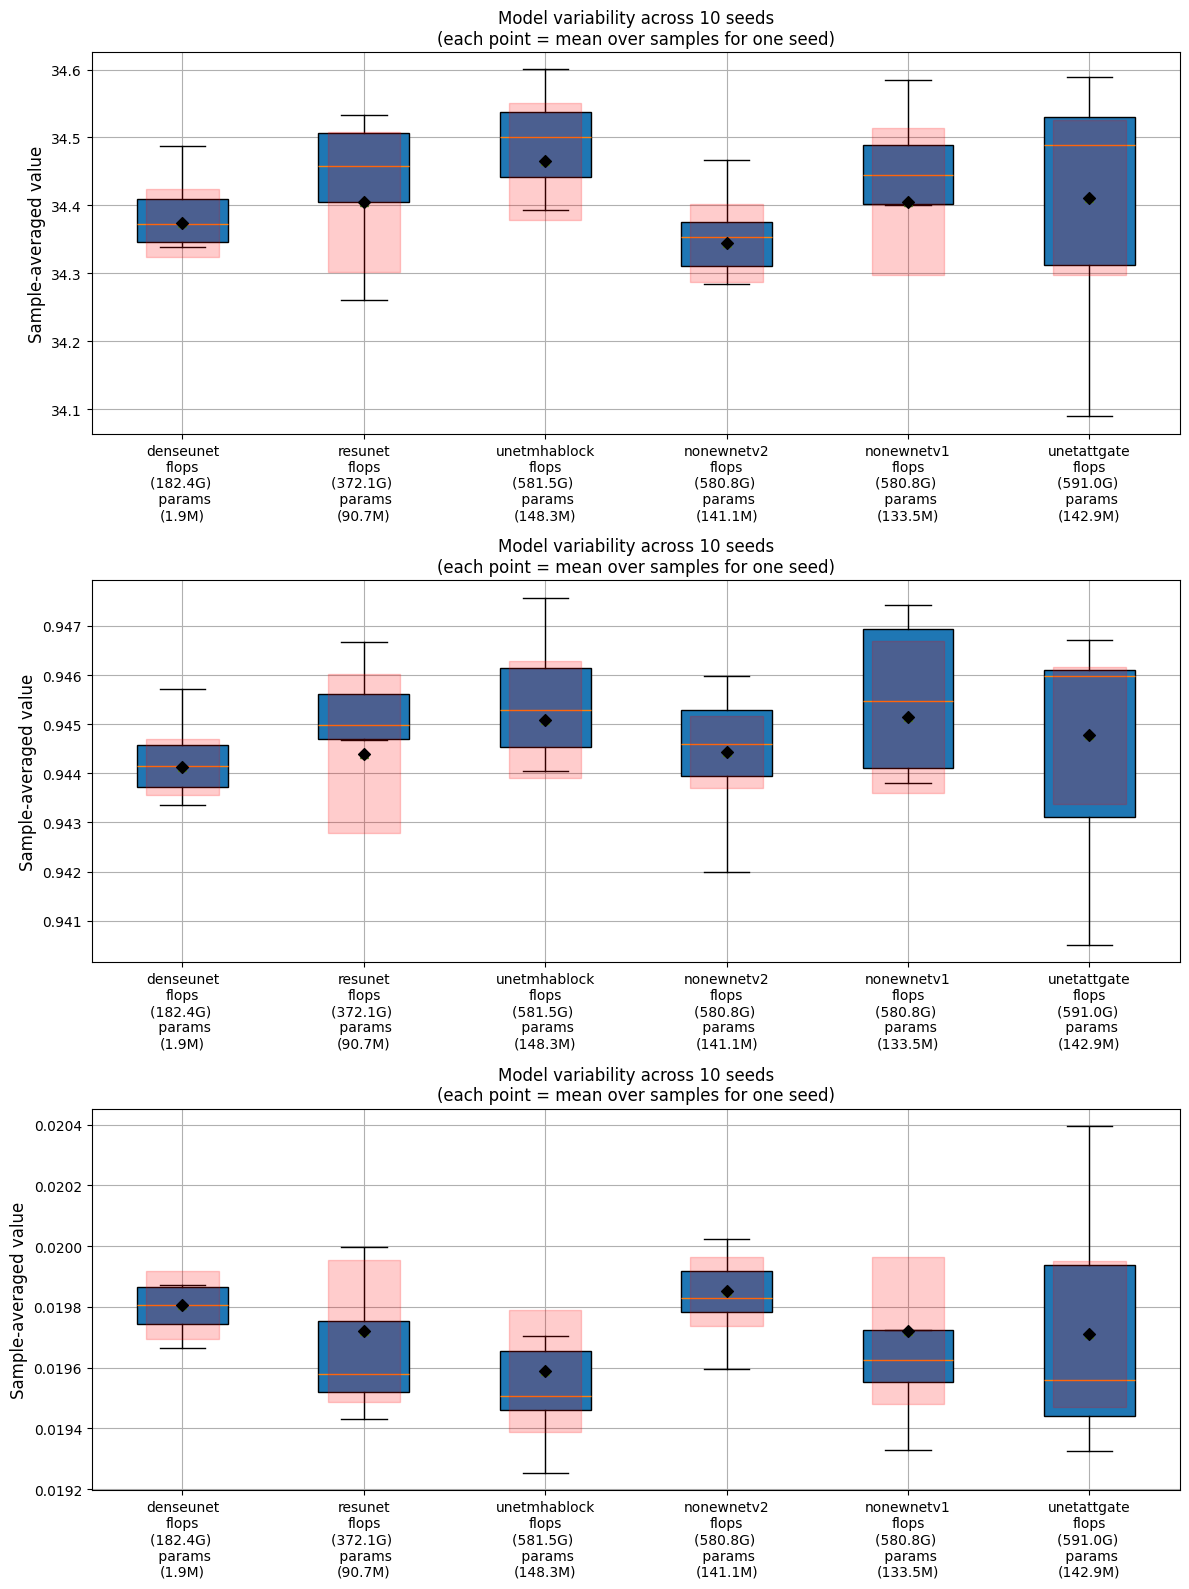
\includegraphics[width=0.75\textwidth]{image/Difference variability 10 seeds.png}
    \caption{Model variability}
    \label{fig:Model variability}
    \vspace{0.5cm}
\end{figure}

This figure illustrates the variability of the network performance across 10 different random seeds using the PSNR, SSIM and RMSE metrics. 
Each boxplot represents the distribution of all the average PSNR obtained for a given seed. 
The red band inside each boxplot corresponds to the 95\% confidence interval of the true mean PSNR.
This confidence interval is computed from the standard deviation across the 10 seeds. 
A shorter red band indicates a more precise estimate of the true mean, meaning there is less uncertainty about the network's average performance.

First, it can be observed that all architectures achieve an average PSNR of approximately 34~dB, which indicates a high reconstruction quality. 
In addition, the interquartile range of each boxplot is around 0.1~dB, showing that the performance is highly consistent across different random initializations.
Based on the average PSNR, the UnetAttBlock architecture appears to provide the best performance.
However, considering the 95\% confidence intervals, the difference between this model and the second-best architecture, ResU-Net, is not statistically convincing.
Indeed, the confidence interval of ResU-Net overlaps with the mean PSNR of the UnetAttBlock model, indicating that the observed difference could simply be due to the variability introduced by the random seeds.

A larger number of experiments, for example using 20 or 30 random seeds, would reduce the width of the confidence intervals and provide a more reliable estimate of the true mean performance.
Nevertheless, performing such an extensive evaluation was beyond the scope of this project.
The main objective was to compare the different architectures under identical conditions while ensuring that the conclusions remained reliable.

Overall, the results show that all investigated architectures achieve very similar reconstruction performance. 
This outcome is not surprising since all these architectures share the same core U-Net design and differ only by relatively minor architectural modifications.
Consequently, when several models provide comparable performance, the simplest architecture should be preferred.
In our case, NoNew-Net offers the best compromise between reconstruction quality, architectural simplicity, and computational cost, making it the most suitable model for the full-sample enhancement task.

\paragraph{Contrast Evaluation}
\mbox{}\\

Finally, the objective of this evaluation is to specifically assess the quality of the contrast enhancement while providing an objective comparison between the different networks. 
To achieve this, two quantitative metrics are used: the Relative Enhancement (RE) and the Contrast Ratio (CR).

\begin{itemize}
    \item \textbf{Relative Enhancement (RE):} This metric measures the relative increase in signal intensity between the pre-contrast segmentation and post-contrast segmentation. 
    It quantifies the degree of enhancement produced by the contrast agent for each acquisition. 
    By comparing the RE computed from the reconstructed images with that of the ground truth, it is possible to evaluate how accurately the network reproduces the expected enhancement.

    \[
    \mathrm{RE} = \frac{\mathrm{mean}_{\mathrm{ROI}_{\mathrm{post}}} - \mathrm{mean}_{\mathrm{ROI}_{\mathrm{pre}}}} {\mathrm{mean}_{\mathrm{ROI}_{\mathrm{pre}}}}
    \]
    where ROI (region of interest) denotes the tumor segmentation region.
    
    \item \textbf{Contrast Ratio (CR):} This metric evaluates the contrast between the segmented lesion and the surrounding background tissue. 
    It measures how distinguishable the lesion is from its environment. 
    A higher contrast ratio indicates better lesion visibility from the surrounding tissue.

    \[
    \mathrm{CR} = \frac{\mathrm{mean}_{\mathrm{ROI}} - \mathrm{mean}_{\mathrm{background}}} {\mathrm{mean}_{\mathrm{background}}}
    \]

\end{itemize}

Both metrics are computed for every sample and for every network, as well as for the corresponding ground-truth samples.

To compare the networks, scatter plots are generated in which the metric values obtained from the reconstructed images are plotted against the ground-truth values.
A linear regression is then fitted for each model using the results of all test samples.
The ideal reconstruction corresponds to the identity line ($y=x$), meaning that the reconstructed metric perfectly matches the ground truth.

By comparing the regression lines of the different models with the identity line, it is possible to assess which model most accurately reproduces the true contrast enhancement.

\begin{figure}[H]
    \centering
    \vspace{0.5cm}
    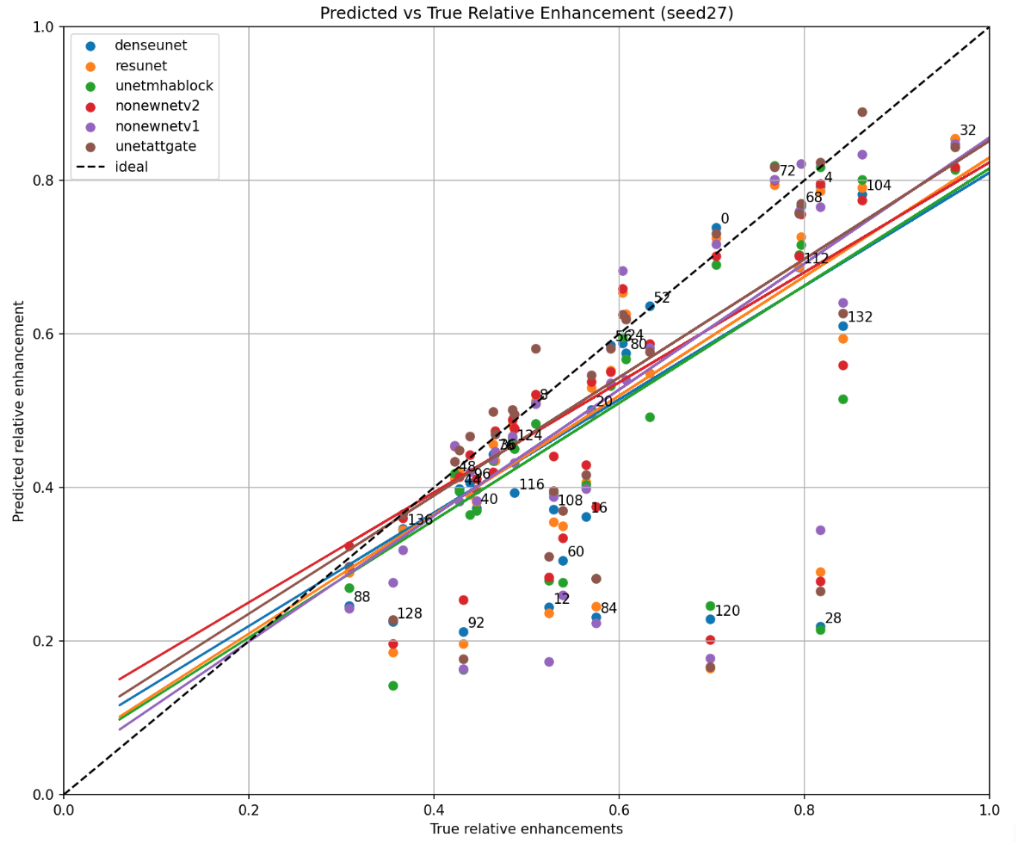
\includegraphics[width=0.75\textwidth]{image/Quantitative relative enhancement.png}
    \caption{Quantitative relative enhancement}
    \label{fig:Quantitative relative enhancement}
    \vspace{0.5cm}
\end{figure}


\begin{figure}[H]
    \centering
    \vspace{0.5cm}
    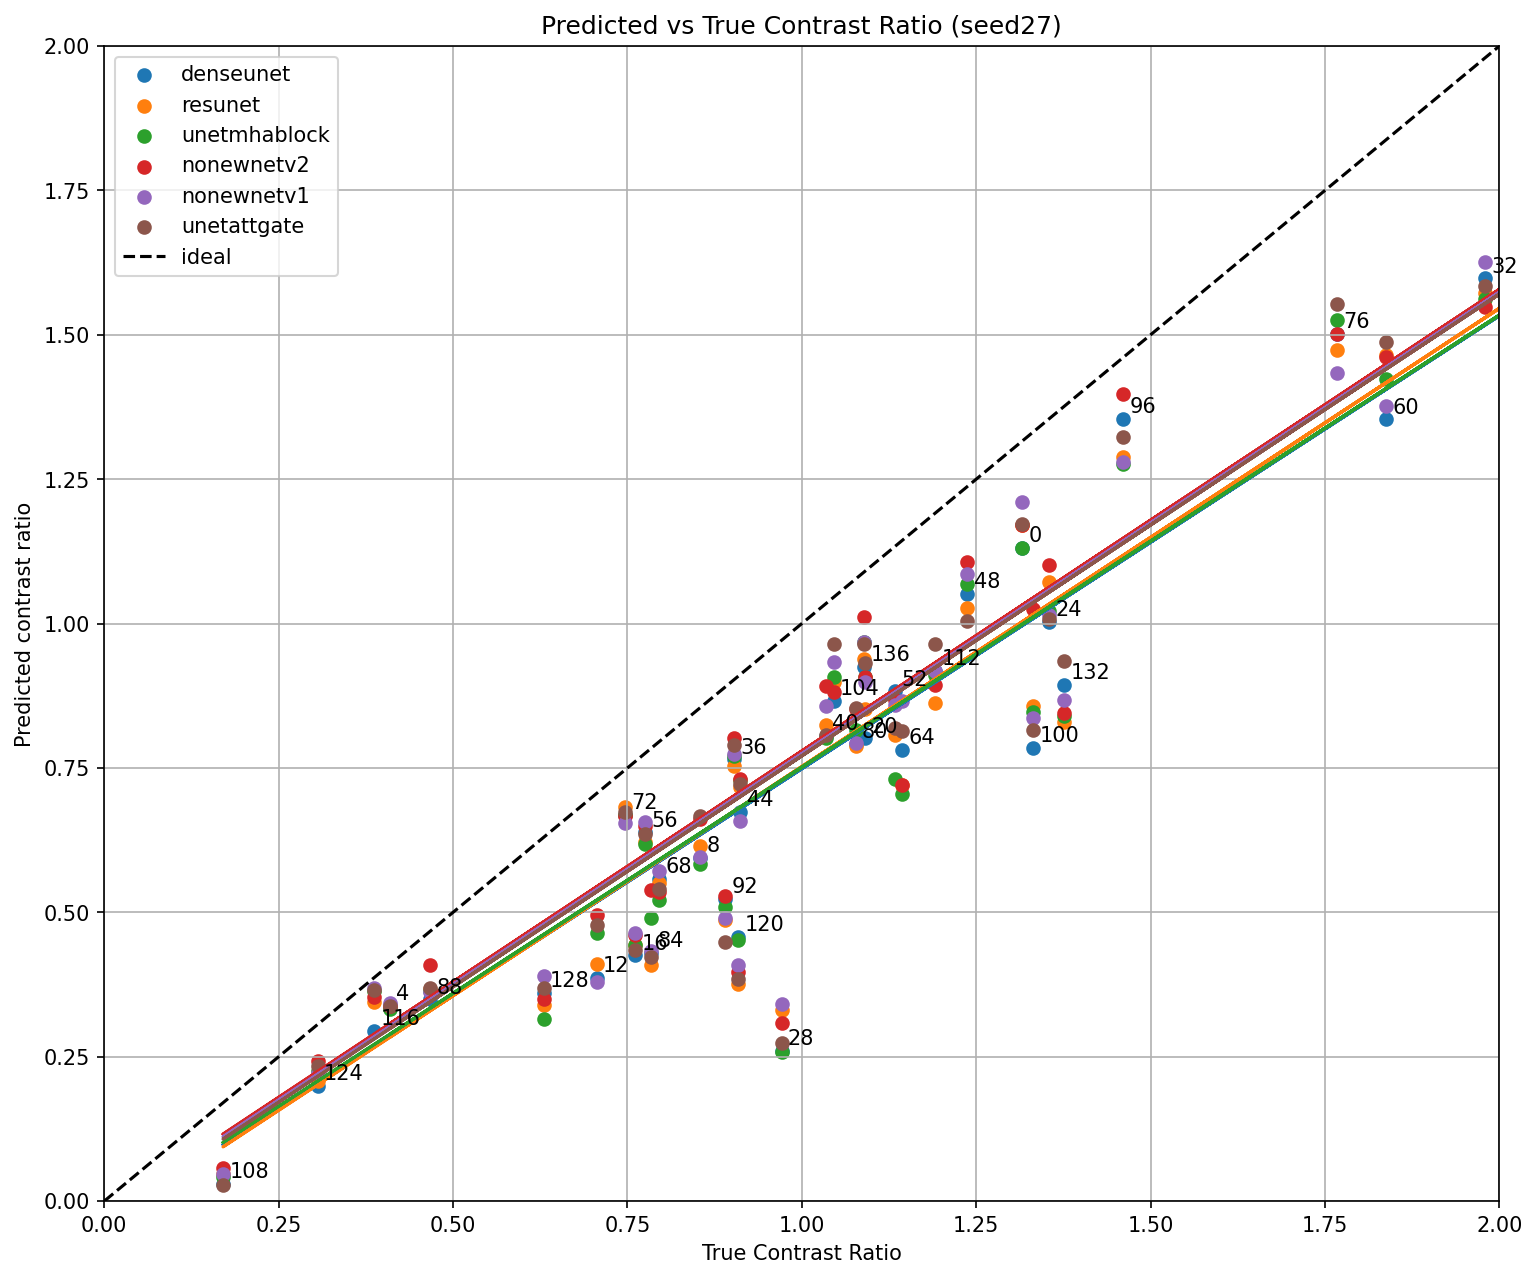
\includegraphics[width=0.75\textwidth]{image/Quantitative contrast ratio.png}
    \caption{Quantitative contrast ratio}
    \label{fig:Quantitative contrast ratio}
    \vspace{0.5cm}
\end{figure}

These figures show, for the relative enhancement and the contrast ratio, the different linear regressions computed over all samples of the test dataset, each regression representing one network.
All the networks are close to the identity line ($y=x$), which means that the contrast enhancement is close to the ground truth.
The fact that all the linear regressions lie below the identity line means that all networks tend to underestimate the contrast.
However, we observe that improving the contrast ratio is more challenging than improving the relative enhancement.
This is expected because the relative enhancement depends only on the average contrast, whereas the contrast ratio depends on both the average contrast and the background intensity. 
Therefore, the model must not only enhance the target contrast but also suppress or maintain a low background level, making the optimization of the contrast ratio more difficult.

However, to compare the performance of the networks for contrast enhancement, as done in the qualitative contrast evaluation, it is necessary to evaluate each model using 10 different random seeds.
The goal was to evaluate the variability of the slope of each linear regression, and of the associated error, with respect to the ground truth.
The ground truth has a slope of 1, since it corresponds to the line ($y=x$).
For each seed, we computed the difference between the estimated slope and the ground truth slope.
A slope closer to 1 indicates that the regression is closer to the ground truth, whereas a slope farther from 1 indicates a larger deviation.

\begin{figure}[H]
    \centering
    \vspace{0.5cm}
    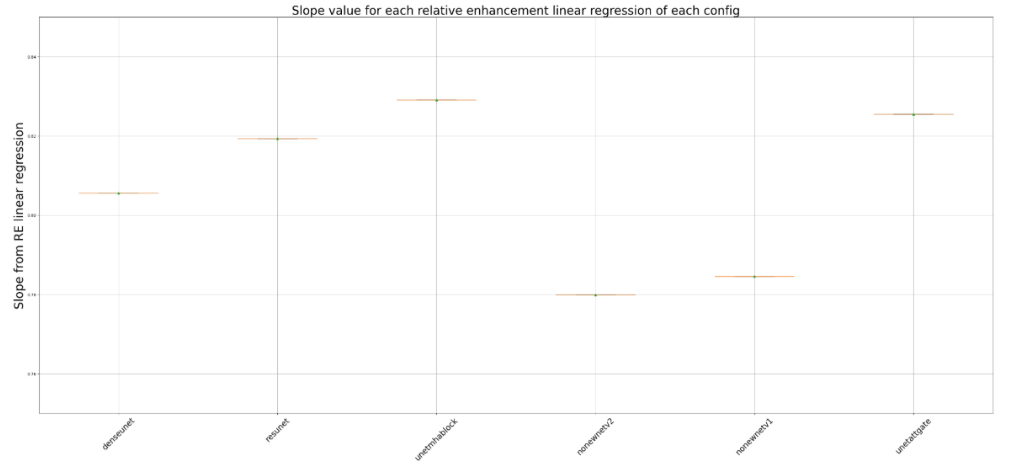
\includegraphics[width=0.75\textwidth]{image/slop contrast ratio.png}
    \caption{Slope contrast ratio}
    \label{fig:Slope contrast ratio}
    \vspace{0.5cm}
\end{figure}

This plot shows the variability of the slope over 10 seeds for the contrast ratio. We can see that the best slope value is 0.86 and that it corresponds to UnetAttBlock.

\begin{figure}[H]
    \centering
    \vspace{0.5cm}
    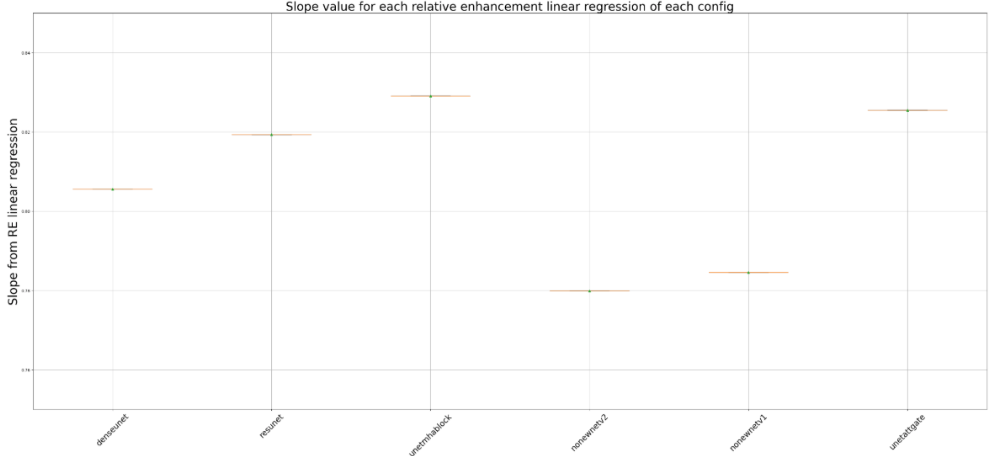
\includegraphics[width=0.75\textwidth]{image/slop relative enhancement.png}
    \caption{Slope relative enhancement}
    \label{fig:slope relative enhancement}
    \vspace{0.5cm}
\end{figure}

This plot shows the variability of the slope over 10 seeds for the relative enhancement. We can see that the best slope value is 0.86 and that it also corresponds to UnetAttBlock.

The next goal was to evaluate the variability of the error of each linear regression.
For each seed, we computed the difference between the estimated CR or RE and the linear regression.
An error closer to 0 indicates that the dispersion error is weak, whereas a dispersion error close to 1 indicates a larger deviation.

\begin{figure}[H]
    \centering
    \vspace{0.5cm}
    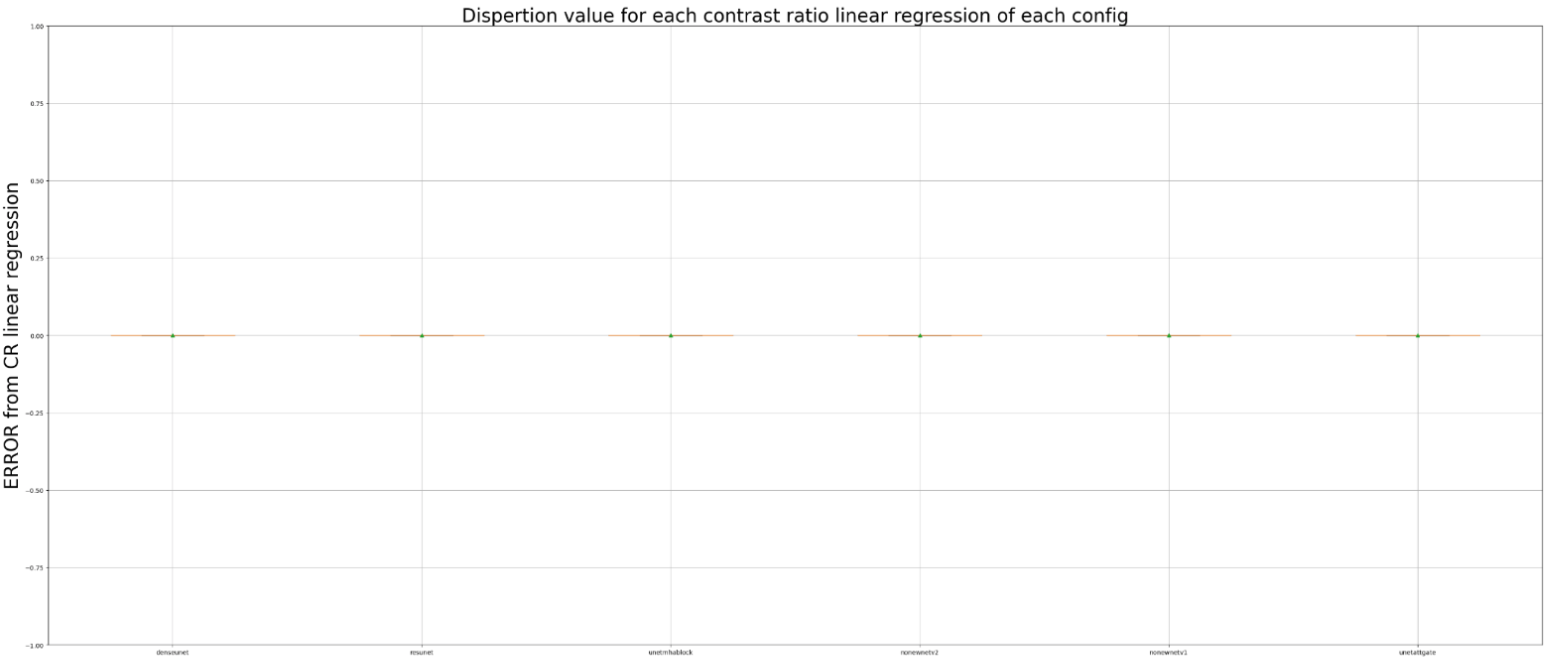
\includegraphics[width=0.75\textwidth]{image/error contrast ratio.png}
    \caption{Contrast ratio dispersion error}
    \label{fig:error contrast ratio}
    \vspace{0.5cm}
\end{figure}

This plot shows the dispersion error over 10 seeds for the CR. We can see that each model has a low dispersion error.

\begin{figure}[H]
    \centering
    \vspace{0.5cm}
    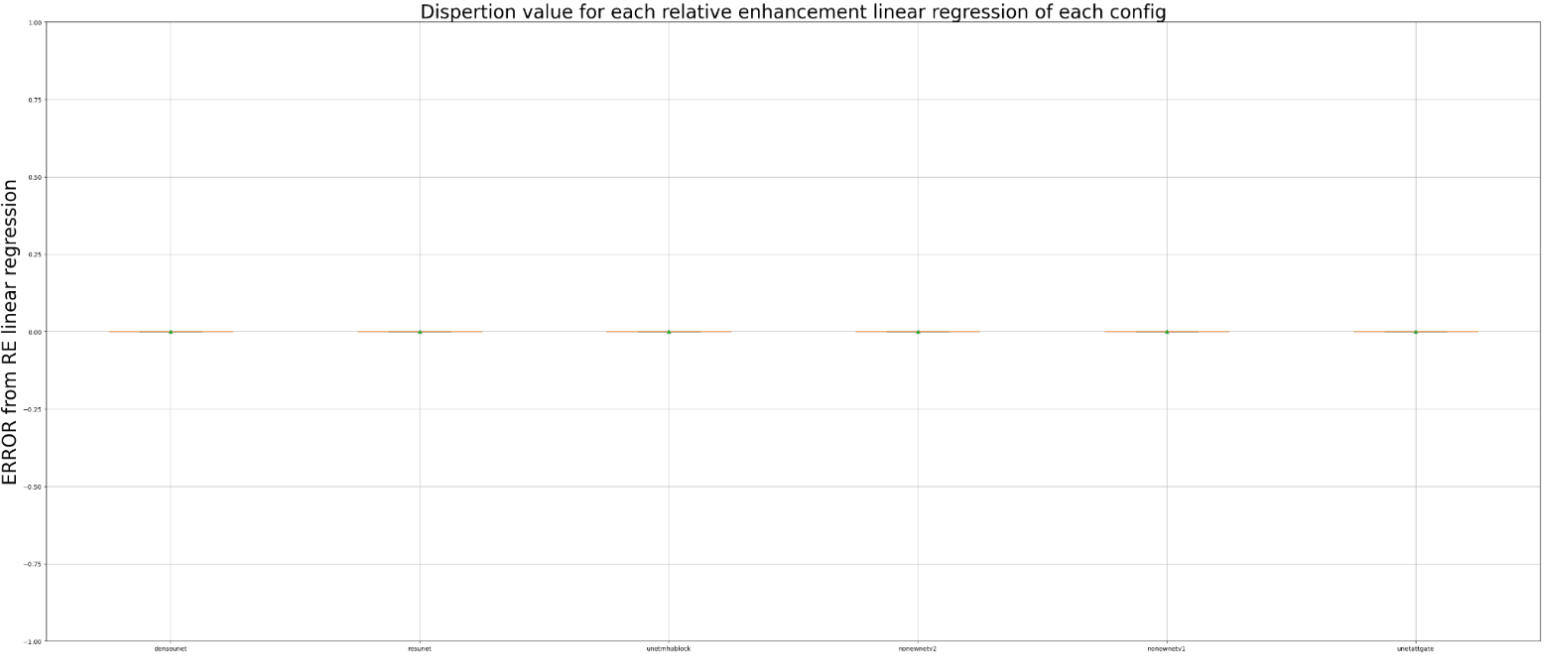
\includegraphics[width=0.75\textwidth]{image/error relative enhancement.png}
    \caption{Relative enhancement dispersion error}
    \label{fig:error relative enhancement}
    \vspace{0.5cm}
\end{figure}

This plot shows the dispersion error over 10 seeds for the RE. We can see that each model has a low dispersion error.


\paragraph{Conclusion on model selection}
\mbox{}\\

For contrast enhancement, it appears that almost all networks achieve acceptable results.
We observe slightly better results for the UnetAttBlock in terms of both relative enhancement (RE) and contrast ratio (CR). 
However, since the differences between the models are relatively small, we reach the same conclusion as in the full-sample analysis: the preferred model is the simplest one that achieves comparable performance. 
In our case, this corresponds to the standard NoNew-Net architecture.

\subsubsection{Other improvements} 

There are additional ways of improving the results without changing the network.

\paragraph{Training with all acquisitions}
\mbox{}\\

A first improvement consisted of using the pre-contrast and all post-contrast acquisitions during training instead of randomly selecting one acquisition per sample at each epoch.
This increased the number of training acquisitions from 139 to 450. 
However, this approach did not improve the model performance. 
A likely explanation is that the additional post-contrast acquisitions contain highly correlated information.
Since the previous training strategy randomly sampled one acquisition at each epoch, the model was already exposed to all acquisitions over the course of training.
Using all of them simultaneously increased the training time considerably (by approximately a factor of four) without providing enough additional diversity to improve the model's generalization performance.

\paragraph{Data augmentation}
\mbox{}\\
Another approach to improving the results was to use data augmentation. Data augmentation helps enforce better generalization by introducing variability in the training data and reducing redundancy, which can also help prevent overfitting.
It was applied directly in the training pipeline on randomly selected acquisitions. 
The augmentation consisted of random flips and rotations along the three main axes.
We observed a slight improvement in relative enhancement (RE), but overall it led to slightly worse results on the full-sample enhancement task.


\subsubsection{Conclusion} 
In this second phase, we explored a new paradigm by using the average of the full acquisition to enhance fast pre-contrast and post-contrast acquisitions.
We also implemented and compared different network architectures in order to evaluate which one was the most efficient for dynamic contrast enhancement.

Overall, most architectures produced good results.
Therefore, we selected the simplest architecture, NoNew-Net, as it offered a good trade-off between performance and simplicity.

We were able to obtain satisfactory results despite the increased complexity of the problem.
Having now fixed the model, the next objective is to address the main internship question: how much the acquisition time can be reduced while still maintaining acceptable performance.

In the third phase, we test different trajectory configurations at different acquisition times to determine
the minimum time required for the network to enhance both the full sample and the contrast.

\subsection{Acquisition Trajectory and Model Optimization} 
\subsubsection{Methodology} 

Now that a realistic experimental setting has been established, better reflecting the conditions encountered in low-field MRI, and that a suitable deep learning network for contrast enhancement has been identified, the project can move to its final phase.
The objective of this last phase is to determine how much the acquisition time can be reduced while still preserving sufficient image quality and contrast enhancement.

To achieve clinically relevant results, all experiments are performed using the spatial resolution of 4.0 × 2.0 × 2.0 mm targeted by Chipiron.
Since the acquisition time directly depends on the acquisition parameters, modifying the spatial resolution also affects the scan duration.

The main objective is therefore to investigate the trade-off between acquisition speed and reconstruction quality. 
This is achieved by progressively reducing the number of acquisition shots and evaluating different sampling trajectory configurations. 
By comparing the enhancement performance obtained with each configuration, we aim to identify the fastest acquisition strategy that still provides accurate contrast enhancement and satisfactory image quality.

\subsubsection{Conception}

First of all, we need to test different acquisition times for each trajectory.
Each acquisition has a resolution of 4.0 × 2.0 × 2.0 mm with a shape of 40 × 160 × 160.
The total number of shots required to acquire the fully sampled k-space is $6400$ ($40 \times 160$).
When we reduce the sampling factor from $1$ to $1/4$, there are four times fewer shots, so the acquisition is four times faster.
The goal is to test different undersampling factors and compare the results in order to determine the limit at which the network can still enhance both contrast and samples while maintaining acceptable performance.

\begin{table}[h]
\centering
\begin{tabular}{c c c c c c c}
\hline
Sampling factor & 1 & 1/4 & 1/8 & 1/16 & 1/32 & 1/80  \\
\hline
Number of shots & 6400 & 1600 & 800 & 400 & 200 & 80\\
Acquisition time & 192~s & 48~s & 24~s & 12~s & 6~s & 2.4~s  \\
\hline
\end{tabular}
\caption{Comparison of acquisition time}
\label{tab:comparison_acquisition_time}
\end{table}

The undersampling factors reported in Table~\ref{tab:comparison_acquisition_time} were deliberately pushed to extreme values to clearly identify the point at which the network is no longer able to produce meaningful enhancements.
Moreover, each undersampling factor was evaluated using three different sampling configurations: \texttt{decay\_cartesian}, \texttt{stack\_of\_radial}, and \texttt{phyllotaxis\_radial}.
Testing each configuration at each undersampling factor also allows us to determine which trajectory gives the best results.

\subsubsection{Validation} 

To validate our results, we reuse the quantitative tests that we had already implemented for the network comparison, except that this time we compare trajectory configurations rather than networks.
As before, we perform two types of quantitative test: the first checks the full-sample enhancement, and the second checks only the contrast enhancement.

\paragraph{Full-sample enhancement quantitative test}
\mbox{}\\

As we did for the network comparison, we use boxplots and train on 10 different seeds to assess the variability of the training at the same time.

\begin{figure}[H]
    \centering
    \vspace{0.5cm}
    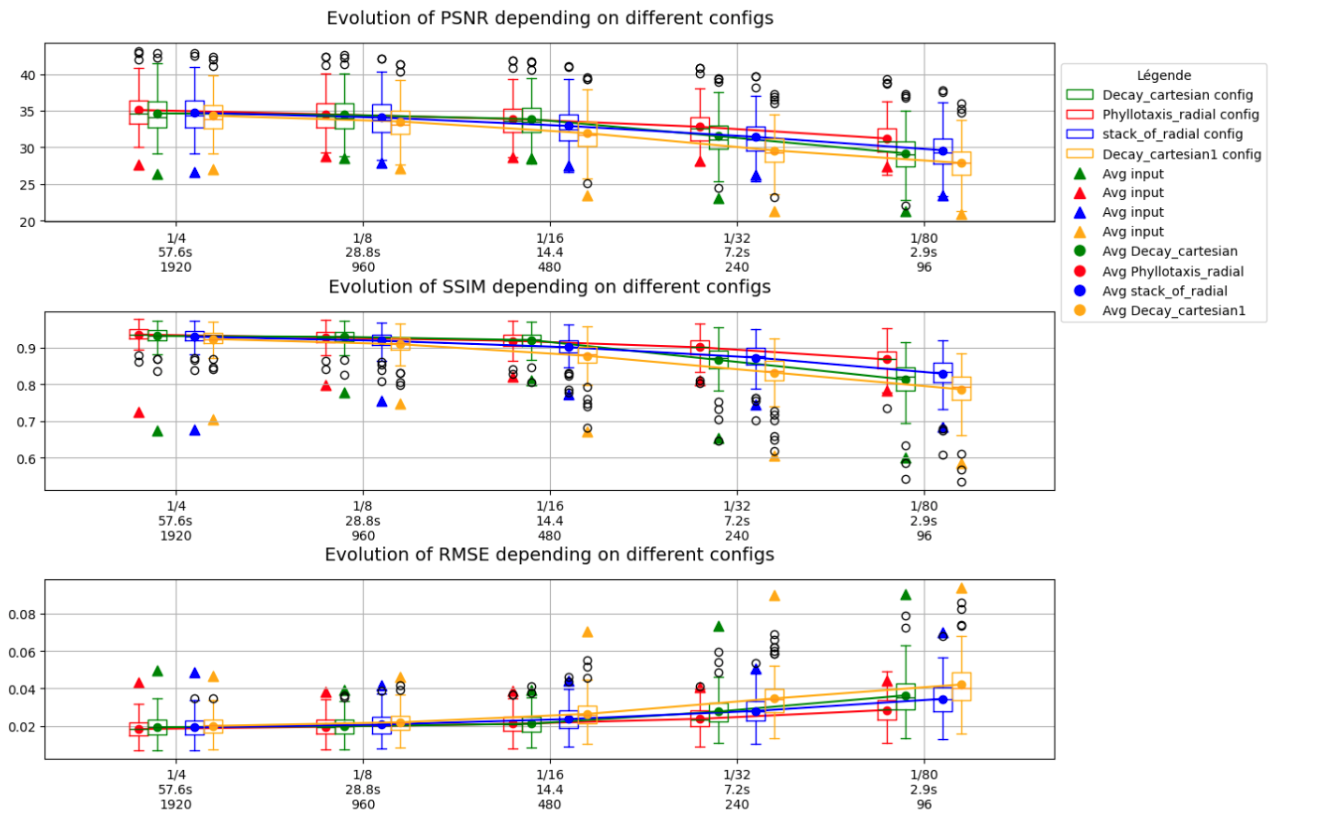
\includegraphics[width=0.75\textwidth]{image/trajectories quantitative test.png}
    \caption{Trajectories quantitative test}
    \label{fig:trajectories quantitative test}
    \vspace{0.5cm}
\end{figure}

In this plot, we observe the boxplots for the three different configurations, which are placed next to each other.
On the y-axis, we report the evaluation metrics, while the x-axis represents the different acquisition times.
The objective is to analyze how the distribution of results evolves with acquisition time for each trajectory configuration.

As expected, the more the acquisition time is reduced, the worse the metrics become.
However, we can see that the difference in metrics between trajectories accelerated with a factor of $1/4$ and a factor of $1/8$ is very small.
This is particularly interesting because, if both acquisitions give similar results but one is twice as fast, then the shorter one would be preferable for our problem.

\paragraph{Contrast enhancement quantitative test}
\mbox{}\\
In the same way as for the full-sample contrast enhancement, we apply the same quantitative analysis used in the network comparison, based on slope and error distribution differences across different seeds for the RE and CR.

\begin{figure}[H]
    \centering
    \vspace{0.5cm}
    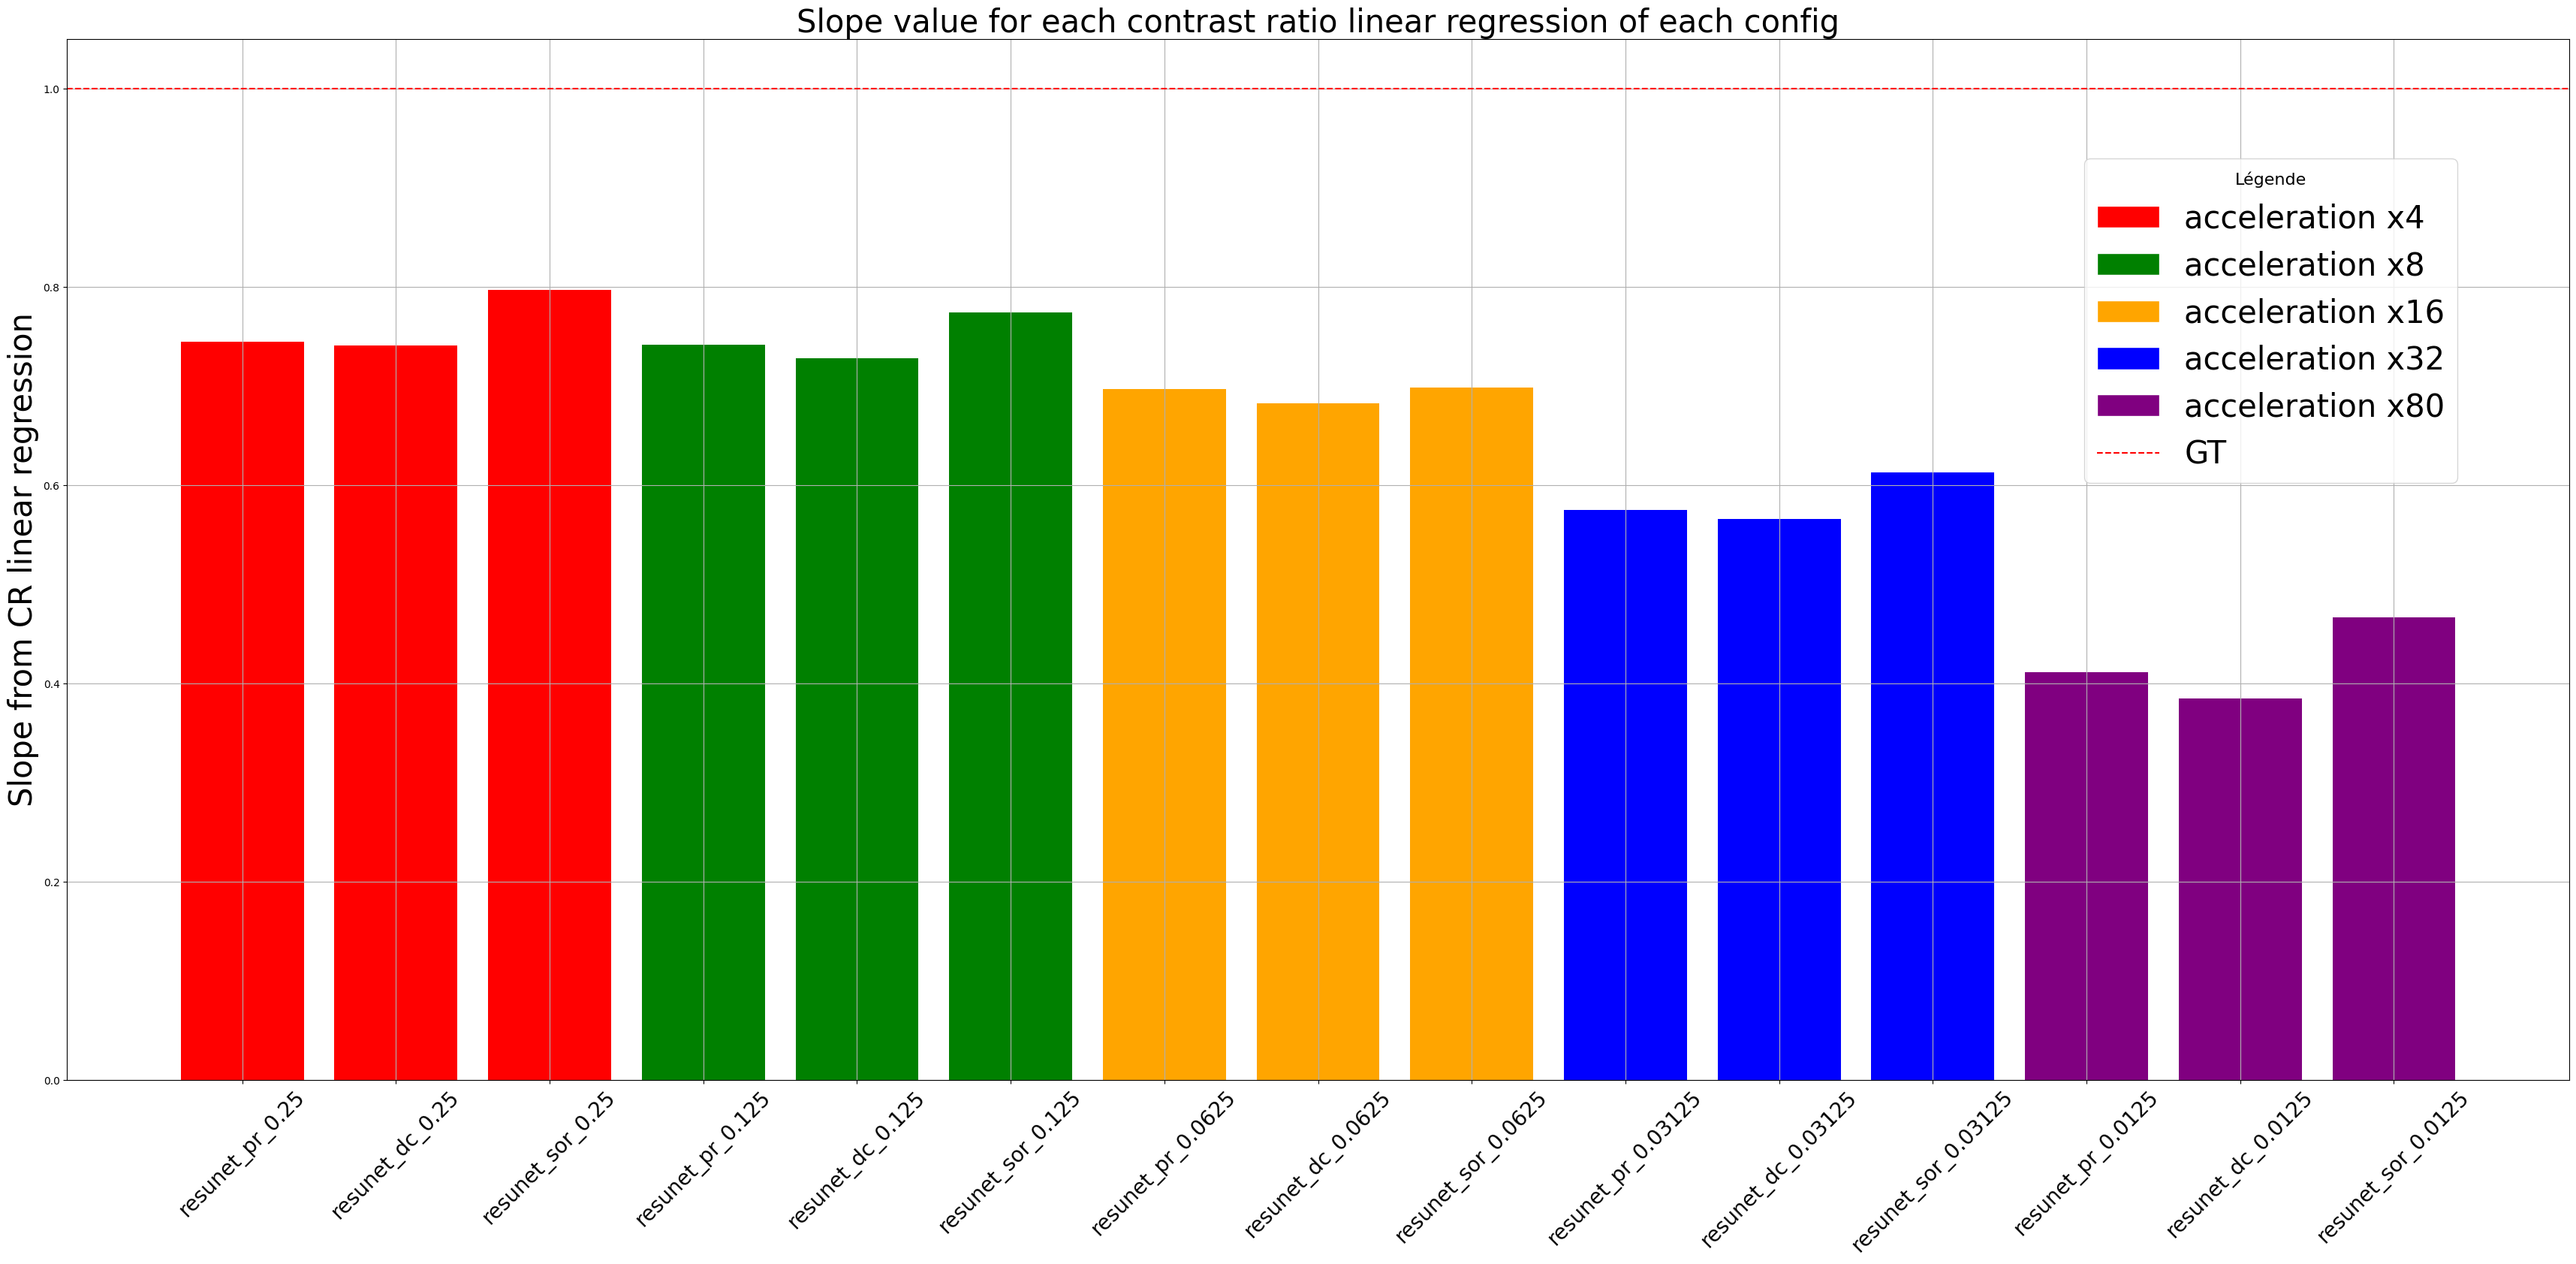
\includegraphics[width=0.75\textwidth]{image/trajectories CR slope.png}
    \caption{trajectories CR slope}
    \label{fig:trajectories CR slope}
    \vspace{0.5cm}
\end{figure}

In this graph, we show the distribution of the slope for each trajectory configuration across 10 different seeds.
Once again, the acquisition factors of $1/4$ and $1/8$ produce very similar results.
However, for the two highest acceleration factors, the metric degrades significantly, indicating that the network is no longer able to effectively enhance the contrast.

\begin{figure}[H]
    \centering
    \vspace{0.5cm}
    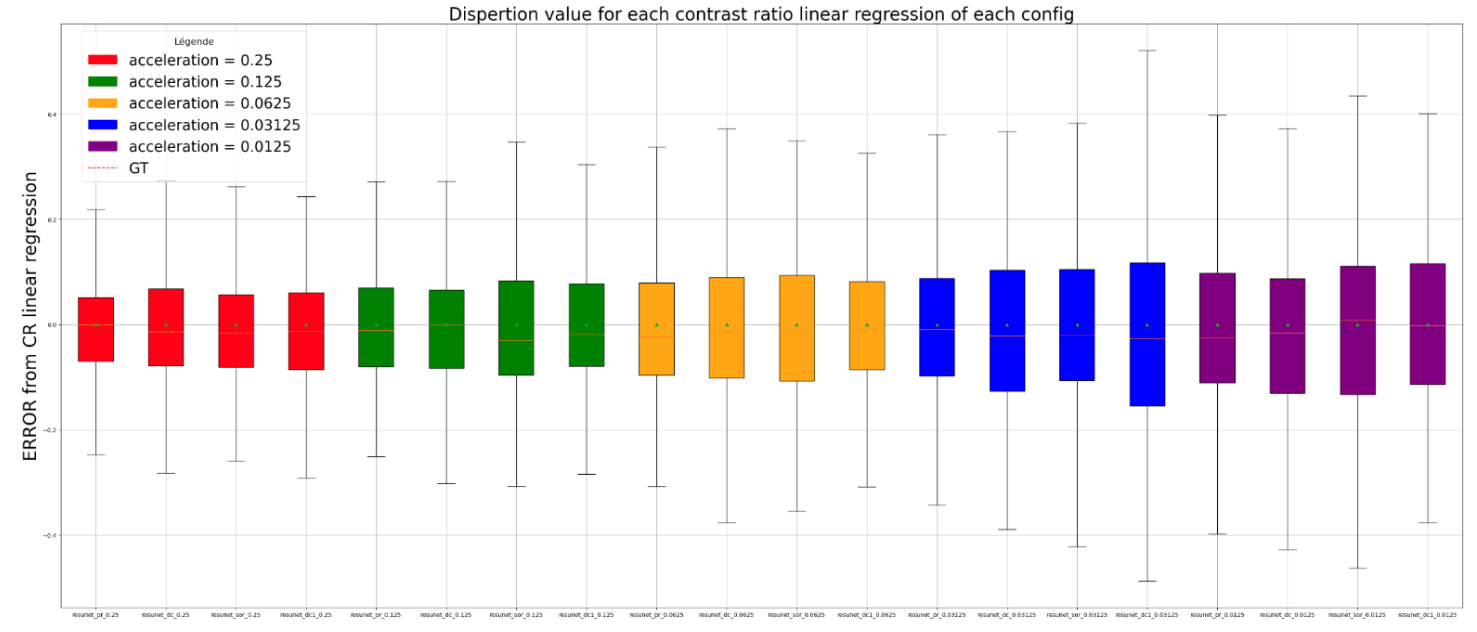
\includegraphics[width=0.75\textwidth]{image/trajectories CR error.png}
    \caption{Trajectories CR error}
    \label{fig:trajectories CR error}
    \vspace{0.5cm}
\end{figure}

This graph shows the distribution of the residual errors between the linear regression and the measured data.
The residuals are centered around zero, indicating that there are relatively few outliers.
Since the residual errors remain small, the estimated slopes can be considered reliable.

\begin{figure}[H]
    \centering
    \vspace{0.5cm}
    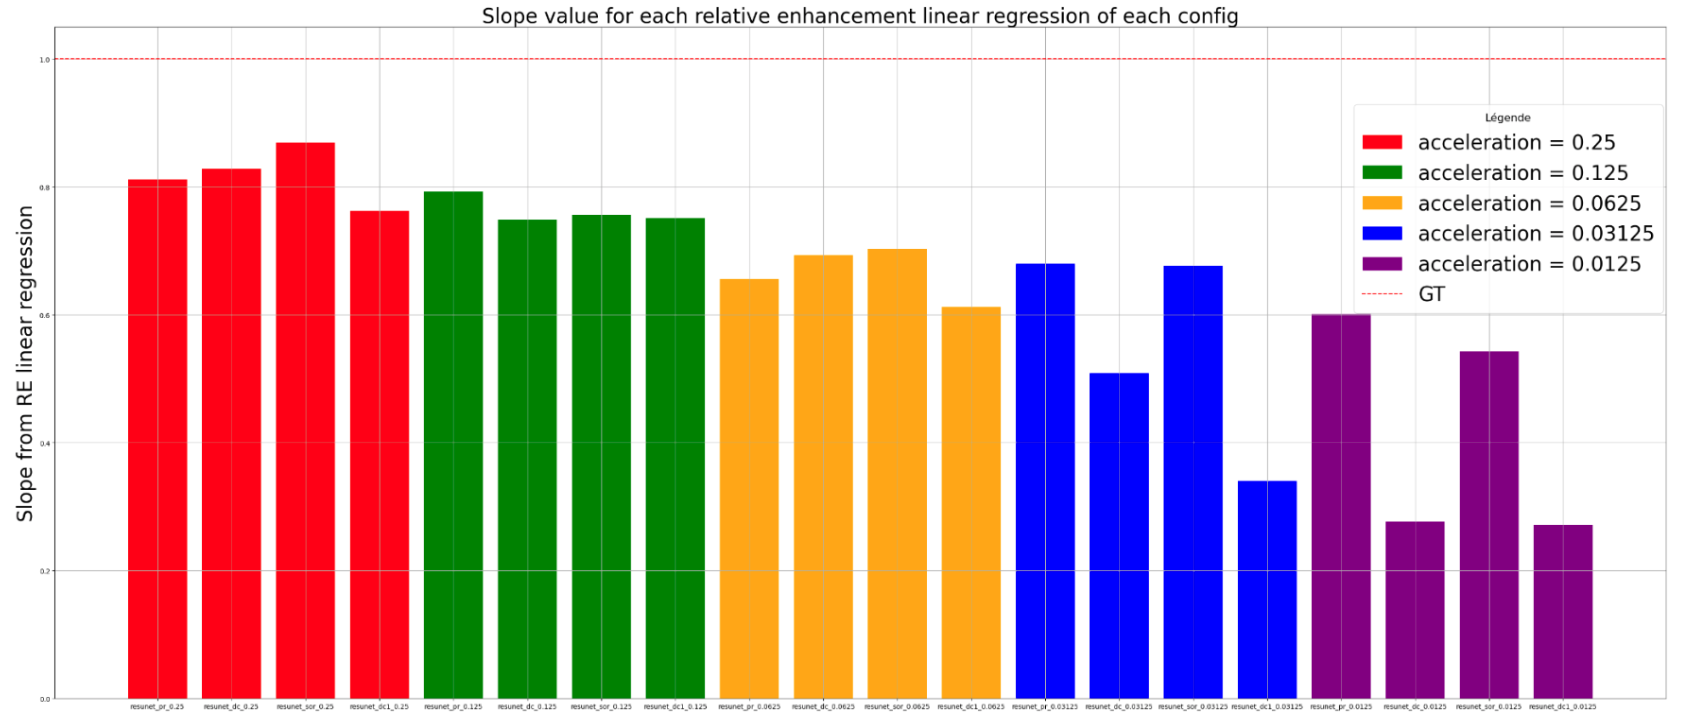
\includegraphics[width=0.75\textwidth]{image/trajectories slope RE.png}
    \caption{Trajectories RE slope}
    \label{fig:trajectories RE slope}
    \vspace{0.5cm}
\end{figure}

This graph is similar to the previous slope distribution.
However, it compares the RE metric instead of the CR metric.
As with the CR metric, the RE slopes for acceleration factors of $1/4$ and $1/8$ are very similar.

\begin{figure}[H]
    \centering
    \vspace{0.5cm}
    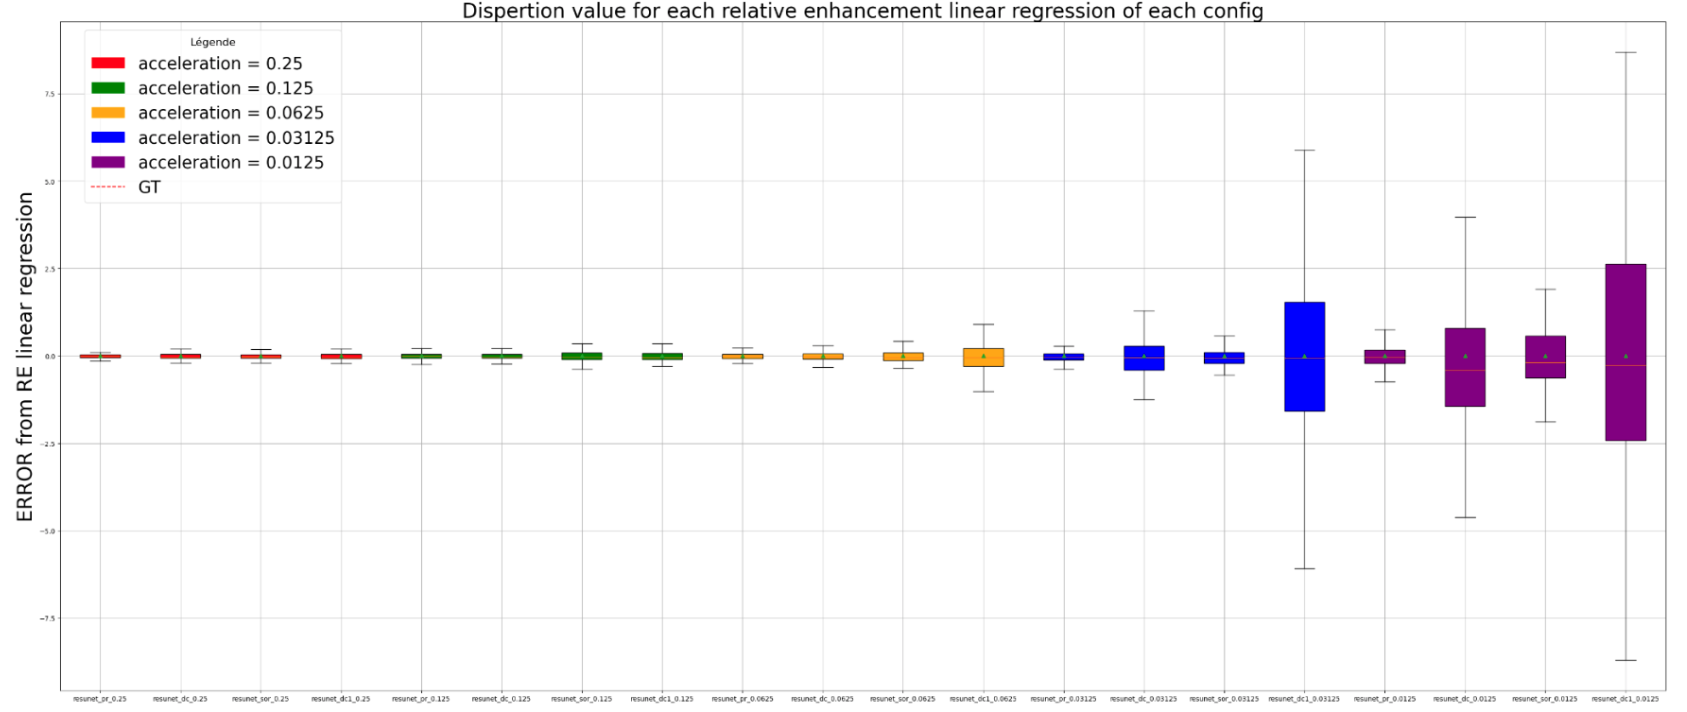
\includegraphics[width=0.75\textwidth]{image/Trajectories relative enhancement config.png}
    \caption{Trajectories RE error}
    \label{fig:trajectories RE error}
    \vspace{0.5cm}
\end{figure}

Finally, this graph shows the residual error associated with the RE slopes. We observe that the error increases rapidly as the acquisition becomes more accelerated.

\subsubsection{Conclusion}

The goal of this final phase was to evaluate three different acquisition configurations and determine how much the acquisition time could be reduced, depending on the configuration, while maintaining sufficient image quality and contrast enhancement.
The three configurations achieve very similar performance, although the \texttt{decay\_cartesian} configuration appears to provide slightly better results, especially for highly accelerated acquisitions.
Moreover, since the $1/4$ and $1/8$ acquisition factors produce very similar results from a physical perspective for each configuration, an acceleration factor of $1/8$ could be selected. 
This corresponds to an acquisition time of approximately 24 seconds, which should be sufficient to monitor the evolution of the contrast over time.
To further validate this choice, a radiologist could assess the minimum image quality required to reliably detect a lesion.
For the purposes of this project, we can therefore conclude that an acquisition time of approximately 24 seconds is an appropriate compromise between acquisition speed and image quality.

\subsection{Difficulties Encountered}
One of the main challenges we encountered during this project was handling outliers in the training dataset.
Indeed, some samples consistently produced very poor enhancement results, regardless of the acquisition configuration.

We investigated these samples to identify possible causes of their poor performance.
However, this proved to be difficult, as there was no single characteristic explaining the failures.
Instead, several correlations appeared to contribute to the degradation.

To better understand these correlations, we performed a Principal Component Analysis (PCA).
This analysis revealed a few weak correlations, notably with the size of the segmented lesion and with small differences in the contrast ratio (CR) between the pre-contrast and post-contrast images. 
Nevertheless, these correlations were not strong enough to draw definitive conclusions, and the PCA analysis remained inconclusive.

As a possible extension of this work, the \textit{MAMA-MIA} dataset also includes a neural network trained for lesion segmentation. 
Evaluating this segmentation model on the enhanced images from our network would be an interesting way to assess whether the image enhancement preserves clinically relevant information. 
In particular, it would allow us to determine whether the segmentation network is still able to accurately identify the lesion after the enhancement process.

\section{Conclusion and Final Assessment}

\subsection{Project Status}

Overall, this project demonstrated the feasibility of using deep learning models to reduce MRI acquisition time while preserving the image quality and contrast enhancement information. 
The feasibility study was structured into three progressive phases, each addressing a more challenging aspect of the reconstruction problem.

The first phase focused on validating whether deep learning models could reconstruct enhanced post-contrast images by using a fully sampled pre-contrast acquisition and a fast post-contrast acquisition.
A complete and flexible pipeline was developed to generate fast acquisitions and test a simple architecture.
The results showed that deep learning models were able to improve accelerated post-contrast images using both pre-contrast and post-contrast acquisitions, while preserving the contrast enhancement information.

The second phase introduced a more realistic acquisition scenario closer to fast low-field MRI conditions.
Instead of relying on fully sampled acquisitions, the models were trained using a single full acquisition containing both pre-contrast and post-contrast information to reconstruct the contrast evolution over time.
Several deep learning architectures were compared, and we found that simpler models consistently achieved the best performance.

The final phase focused on optimizing the acquisition strategy by evaluating different undersampling configurations. 
The objective was to determine how much the acquisition time could be reduced while maintaining sufficient image quality and contrast dynamics. 
The results demonstrated that the acquisition time could be reduced by a factor of 4 to 8 while preserving image quality comparable to the original acquisition.
For the 10~mT Chipiron low-field MRI system, this corresponds to acquisition times between 24~s and 48~s, which could enable the monitoring of contrast dynamics in malignant lesions.

Overall, this work demonstrates that deep learning can significantly reduce MRI acquisition time while maintaining image quality and dynamic contrast enhancement.

\subsection{Future Work and Continuation}
Future work will involve collaborating with a radiologist to determine how much the MRI acquisition can be accelerated while still allowing a reliable clinical diagnosis.
Indeed, at this stage, it is difficult to define an acceptable acquisition time without the expertise of a radiologist.

Moreover, to further validate this feasibility study, the proposed approach will need to be evaluated on real clinical cases rather than only on retrospective datasets.

The objective of future clinical studies will be to assess the performance of the proposed method in a real-world setting. 
The first clinical study is expected to take place within the next year and will include 20 patients who will undergo MRI acquisition with gadolinium contrast agent administration. 
The initial objective will be to verify that the accelerated acquisitions can be successfully reconstructed and enhanced using the proposed approach.

In a subsequent clinical study, the focus will shift toward evaluating the ability of the method to accurately capture contrast dynamics, particularly the wash-in and wash-out phases, which are essential for diagnosis.

\subsection{Contribution to the Company}

The training pipeline and the developed deep learning models will be made available to the company through a GitHub repository, providing a reusable framework for future developments and experiments.

This feasibility study demonstrated that deep learning approaches have the potential to reduce MRI acquisition time while preserving image quality and contrast enhancement dynamics. 
The results provide the company with an initial validation of this approach and a foundation for further clinical evaluation.

The next step will be to validate these findings in a hospital environment using real patient data. 
Clinical studies will be conducted to assess whether the proposed method can successfully reconstruct accelerated acquisitions and preserve the contrast dynamics required for clinical analysis.

% what will they do after
\subsection{Quality Assessment of the Work}

\section{Appendices}
\subsection{CV Before the Internship}

\includepdf[pages=-]{image/CV English 2025_2026.pdf}
\subsection{CV After the Internship (Final Year Engineering)}

\includepdf[pages=-]{image/CV Paris (may 2026).pdf}
\subsection{Career Prospects}
% talk about the idea of doing a phd
I really enjoyed this internship, and I particularly like working on deep learning applied to medical imaging.
I would like to continue working in this area, which is computer vision.
That is why my next goal would be to do a PhD in computer vision, more specifically in deep learning applied to medical imaging.
Indeed, doing a PhD would give me more time to explore in greater depth each of the methods that I use in deep learning.
Moreover, my goal is to be skilled and very precise in that domain, because I want to become specialized in deep learning.

Finally, doing a PhD in computer science applied to medical images would allow me to pursue my goal, which is to work in healthcare.
I think that using AI algorithms in medical imaging is the future of diagnostics.
When I started my Master's degree at ECE Paris in the field of health and technology, I chose this specialty because I wanted to bring a purpose to my future work, and I knew that healthcare was a field with a lot of innovation.
I am following my goal, which is to work in healthcare innovation.

\bibliographystyle{unsrt}
\bibliography{references}

\end{document}